\chapter{Experimenty}\label{cha:experimenty}

V této kapitole prezentujeme návrhy nových architektur hlubokých neuronových sítí pro extrakci melodie a jejich výsledky na validační množině. Modely byly trénované nad datasetem MedleyDB. Data byla rozdělena na trénovací, validační a testovací množinu tak, aby skladby od jednoho interpreta náležely právě do jedné z množin. Využili jsme existujícího rozdělení používaného v článcích \cite{Bittner2017} a \cite{DBasaranSEssid2018}, validační i testovací výsledky jsou tedy díky tomu porovnatelné s výsledky uvedenými v článcích.

Navrhované sítě jsou koncipovány jako nové způsoby výpočtu funkce salience. Cílem je ze vstupního okna signálu získat ohodnocení znějících tónů, přičemž v ideálním případě nejvyšší ohodnocení bude mít nejvýraznější tón --- tedy ten, který nese melodii. Naopak tóny doprovodu a frekvenční složky perkusí by měly být v této výstupní reprezentaci co možná nejvíce upozaděny. Zdůrazníme, že těžištěm této práce je odhad výšky tónů; pro detekci melodie používáme pouze jednoduchou metodu práhování. Po výpočtu funkce salience také nepoužíváme žádný modul pro vyhlazování predikcí v čase, pouze vybíráme maximální hodnotu výstupu v každém časovém okně. Tímto zaměřením pouze na výpočet funkce salience je práce podobná práci \cite{Bittner2017}.

Pro výpočet salienční funkce porovnáváme tři různé architektury inspirované pracemi \cite{Kim2018}, \cite{Oord2016} a \cite{Bittner2017}, tyto architektury se pokoušíme systematickým hledáním přizpůsobit pro účel extrakce melodie pomocí vhodných úprav jak v jejich topologii tak nastavením hyperparametrů. První práce popisuje architekturu CREPE, původně navrženou pro sledování výšky tónů v jednohlasých nahrávkách. Architektura WaveNet popsaná týmem \cite{Oord2016} je složena z dilatovaných konvolucí a původně určena pro generování lidské řeči, autoři však zmiňují její možné použití i pro přepis řeči. \cite{Bittner2017} používá speciální vstupní reprezentaci signálu, kterou zpracovává pomocí hluboké konvoluční sítě, její práce se zabývá kompletním přepisem nahrávek i přepisem melodie. 

% Pro detekci melodie pak srovnáváme jednoduchou metodu práhování a složitější samostatný modul, založený na hlubokých neuronových sítích.

\section{Architektura CREPE}\label{sec:crepe}

První sada experimentů se zakládá na architektuře popsané v článku od \cite{Kim2018} použité pro sledování jednohlasu. Jak blíže popisujeme v kapitole \nameref{cha:souvisejici}, cílem sledování jednohlasu je určit konturu základní frekvence melodického nástroje v jednohlasé nahrávce. Tato nahrávka se zpravidla skládá ze směsi čistého signálu hlasu a šumu v pozadí. Pokud však rozšíříme pojem šumu v pozadí tak, aby zahrnoval i melodický doprovod, pak dostáváme polyfonní signál, tedy vstupní signál pro metody extrakce melodie.

Jinými slovy je sledování jednohlasu speciálním případem extrakce melodie a tudíž přinejmenším stojí za zkoušku pokusit se tuto architekturu pro extrakci využít. Mimo to jednohlasé stopy často obsahují přeslech ostatních nástrojů, pokud nahrávka vznikala při společném hraní ve studiu, tudíž by model trénovaný na vícehlasých mixech mohl být robustní vůči tomuto druhu rušení. 

\begin{figure}[h]\centering
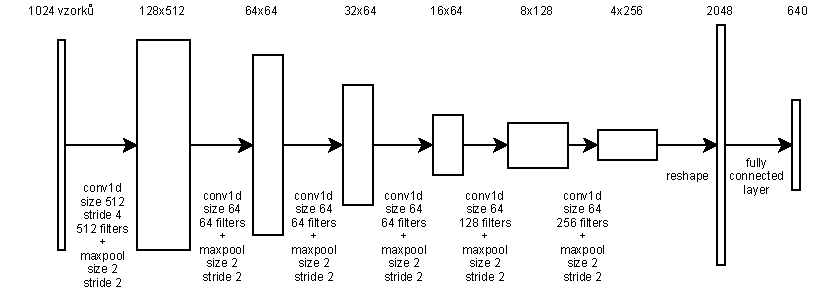
\includegraphics[width=\textwidth,height=\textheight,keepaspectratio]{../img/crepe_arch_grey}
\caption{Diagram architektury CREPE, multiplikační koeficient 16x.}
\label{obr:wavenet_dilated}
\end{figure}

Architektura CREPE se skládá ze šesti konvolučních a pooling vrstev, pro regularizaci používá batch normalization (\cite{Ioffe2015}) a dropout (\cite{Sutskever2014}) po každé konvoluční vrstvě, jako nelineární aktivace je použita funkce ReLU. Po konvolucích následuje výstupní plně propojená vrstva, jako finální aktivační funkce je použita sigmoida. Vstupem modelu je okno o velikosti 1024 vzorků jednokanálového audio signálu, převzorkovaného na 16 kHz. Před první konvolucí je signál normalizován tak, aby každé jednotlivé vstupní okno mělo střední hodnotu 0 a směrodatnou odchylku 1 --- aplikováním normalizace o signálu neztratíme pro nás důležité informace, protože výška tónu nezávisí na absolutním posunu signálu nebo na jeho amplitudě. Naopak tento krok zrychluje trénování, protože síť se nemusí učit být vůči těmto rozdílům v datech invariantní. Celková struktura a podrobnější popis modelu je naznačen na obrázku.

Výsledný vektor s 640 složkami aproximuje pravděpodobnostní rozdělení pro hodnotu výšky tónu melodie uprostřed vstupního okna, přičemž tento vektor pokrývá rozsah od noty $C_{-1}$ po $G_{9}$, mezi dvěma sousedními predikovanými výškami je tudíž vzdálenost 20 centů. Výšky tónů v centech označíme $\cent_1, \cent_2, \dots, \cent_{640}$. Rozsah výstupního vektoru tedy bezpečně pokrývá obvyklé rozsahy hlasů hudebních nástrojů a na jednu notu připadá 5 složek (tónů) výsledného vektoru.

    $$\cent(f) = 1200 \log_2{\frac{f}{f_{\mathrm{ref}}}}$$

Pro trénování modelu potřebujeme také cílové diskrétní pravděpodobnostní rozdělení základní frekvence tónu. Jako cílovou pravděpodobnostní funkci použijeme normální rozdělení se střední hodnotou v bodě cílové základní frekvence $\cent(f_{\mathrm{ref}})$ a se směrodatnou odchylkou 25 centů. Toto rozdělení diskretizujeme tak, aby měl cílový vektor stejné dimenze jako odhadovaný.

    $$y_i = \frac{1}{\sqrt{2 \pi \sigma^2}}\exp{(-\frac{(\cent_i - \cent_{\mathrm{ref}})^2}{2 \sigma^2})}$$

Převod z pravděpodobnostní reprezentace výstupního vektoru na konkrétní hodnotu výšky noty provedeme pomocí výpočtu střední hodnoty výstupní distribuce. Jelikož by při výpočtu střední hodnoty ale hodnotu výsledné výšky tónu ovlivňoval i doprovod, který se na výstupním vektoru objevuje, počítáme střední hodnotu pouze z okolí maxima výstupu. Tím zajistíme, že získáme střední hodnotu gaussiánu náležícímu pouze jednomu tónu.

    $$ \left. \hat{\cent} = \sum_{\scaleto{i, \lvert \cent_i - \cent_m \rvert < 50}{8pt}} {\hat{y}_i \cent_i} \middle/ \sum_{\scaleto{i, \lvert \cent_i - \cent_m \rvert < 50}{8pt}} \hat{y}_i \right., m = \mathrm{argmax}_i(\hat{y}_i)$$

Optimalizovaná ztrátová funkce modelu (loss funkce) $\mathcal{L}(\mathbf{y}, \mathbf{\hat{y}})$ se počítá jako cross-entropy mezi vektorem cílových pravděpodobností $y$ a výstupním vektorem $\hat{y}$.

    $$\mathcal{L}(\mathbf{y}, \mathbf{\hat{y}}) = \sum_{i = 1}^{640}{(-y_i\log\hat{y}_i - (1-y_i)\log(1-\hat{y_i}))}$$

Optimalizace probíhá pomocí algoritmu Adam \citep{Kingma2014} s parametrem learning rate $0.0002$.

\begin{table}[h!]

\centering
    \begin{tabular}{l@{\hspace{1.5cm}}rrrrrrr}
    \toprule
    {}         &  \textbf{1.}   &  \textbf{2.}  &  \textbf{3.}  &  \textbf{4.}  &  \textbf{5.}   &  \textbf{6.}  &  \textbf{Celk. parametrů} \\
    \midrule
    CREPE 4x   &  128  &  16  &  16  &  16  &  32   &  64  &  $558\,240$ \\
    CREPE 8x   &  256  &  32  &  32  &  32  &  64   &  128 &  $177\,1200$ \\
    CREPE 16x  &  512  &  64  &  64  &  64  &  128  &  256 &  $6\,163\,200$ \\
    \bottomrule
    \end{tabular}

\caption{Počty filtrů v konvolučních vrstvách v architektuře CREPE v závislosti na multiplikačním koeficientu.}\label{tab:crepe_dimensions}

\end{table}

% rozepsat:
% - obhajoba raw signálu

% diskuze:
% - převzorkování na 16kHz
% - normalizace vstupu
% - formulace jako klasifikační úloha, nikoli regresní
% - je lepší odhadovat opravdové pravděpodobnostní rozdělení a nebo jejich škálované? (přijde mi, že kvůli sigmoid aktivaci bude jednodušší 1.0 = Truth, protože ty vstupní logity do sigmoid aktivace můžou být crazyshit velký)
% - crepe model - např. nedává vůbec smysl velikost kernelu 64 v posledních vrstvách, zbytečně se tam přidávají nuly jako padding
% - ukázat vizualizaci první vrstvy

V následujících experimentech se zaměříme nejprve na replikaci výsledků pro sledování jednohlasu, následně v základním nastavení model spustíme i pro melodická data. Poté prozkoumáme nejvhodnější nastavení cílové reprezentace refereční anotace melodie, na základě které se síť učí. Tyto experimenty budou užitečné následně i pro další testované architektury, jelikož způsob reprezentace melodie využíváme ve všech experimentech práce stejný. V předposledním experimentu prozkoumáváme vliv zvětšení kontextu, který má síť k dispozici pro predikci výšky tónu. V závěru se pokusíme vyřešit autory zmíněný problém architektury, který se týká odhadu tónů, které mají vysokou frekvenci.

\subsection{Replikace výsledků CREPE}

Abychom ověřili správnost implementace architektury CREPE pro sledování jednohlasu, spustíme model na syntetických, jednohlasých datech MDB-stem-synth, která byla zvěřejněná spolu s článkem od \cite{Salamon2017}.

Na rozdíl od článku \cite{Kim2018}, ve kterém autoři používají pro celkové vyhodnocení architektury pětinásobnou křížovou validaci, jsme použili pouze jednu trénovací a testovací množinu. Zásadní rozdíly mezi implementacemi modelu jsme na základě článku a veřejně dostupného kódu neobjevili.

Po jedné epoše trénování model dosáhl na testovací množině $98.6\%$ přesnosti odhadu výšky. \cite{Kim2018} uvádí přesnost modelu $97\%$. V jejich případě jde o průměrný výsledek pěti nezávislých běhů trénování a testování na různě rozdělených datových množinách. Rozdíl mezi dosaženými přesnostmi tedy přičítáme odlišné evaluační strategii. Přehled výsledků je uveden v tabulce \ref{tab:crepe_replicate}\footnote{Při replikaci experimentu jsme narazili na důležitost správného promíchání dat. Framework Tensorflow použitý pro trénování promíchává data vždy pomocí bufferu pevné velikosti pro dvojice vstupů a cílových výstupů. V praxi je však potřeba buď nastavit buffer na velikost větší než je celková velikost datasetu, a nebo implementovat vlastní míchání přes všechna dostupná data. Při nedostatečně promíchaných datech totiž trénovací dávka (batch) není reprezentativní pro celý dataset, ale pouze pro jeho podmnožinu, což se negativně projevuje kolísající validační přesností modelu.
}

\begin{table}[h!]

\centering
    \begin{tabular}{llrr}
    \toprule
    Metrika & Práh & Průměrná hodnota & Hodnota \cite{Kim2018} \\
    \midrule
    RCA & 50 centů & 0.988 & 0.970 \\
    RPA  & 50 centů & 0.986 & 0.967 \\
    RPA  & 25 centů & 0.975 & 0.953 \\
    RPA  & 10 centů & 0.937 & 0.909 \\
    \bottomrule
    \end{tabular}
\caption{Výsledky pokusu o replikaci architektury CREPE pro sledování jednohlasu. Přesnosti nejsou přímo srovnatelné kvůli různým evaluačním strategiím.}\label{tab:crepe_replicate}

\end{table}

\subsection{CREPE pro extrakci melodie}

Jako první experiment extrakce melodie z polyfonních dat spustíme nezměněnou architekturu CREPE, v následujících experimentech se tuto baseline pokusíme překonat. Abychom urychlili trénování následujících experimentů, přesnost určíme pro sítě s různou kapacitou. Pokud se výsledky při různých kapacitách nebudou příliš lišit, můžeme experimenty provádět s architekturou s nižší kapacitou a tím snížit trénovací čas. Kapacity upravíme pomocí multiplikačního koeficientu počtu filtrů u všech konvolučních vrstev, počty filtrů jsou uvedeny v tabulce \ref{tab:crepe_dimensions}.

% TODO: diskuse o under a overfittingu

\begin{table}[h!]

\centering
    % \begin{tabular}{l@{\hspace{1.5cm}}rr}
    % \toprule
    % \textbf{Model}      &  \textbf{RPA}    &  \textbf{RCA} \\
    % \midrule
    % CREPE 4x   &  0.634  &  0.753 \\
    % CREPE 8x   &  0.661  &  0.766 \\
    % CREPE 16x  &  0.666  &  0.771 \\
    % \bottomrule
    % \end{tabular}
% \begin{tabular}{lrrr}
% \toprule
% {} &  Raw Pitch Accuracy &  Raw Chroma Accuracy &  Voicing Accuracy \\
% \thead{Multiplikátor \\ kapacity sítě} &                     &                      &                   \\
% \midrule
% \textbf{4                          } &               0.634 &                0.753 &             0.534 \\
% \textbf{8                          } &               0.661 &                0.766 &             0.534 \\
% \textbf{16                         } &               0.666 &                0.771 &             0.534 \\
% \textbf{32                         } &               0.656 &                0.753 &             0.591 \\
% \bottomrule
% \end{tabular}

\begin{tabular}{rrr}
\toprule
Mult. koef. kapacity &   RPA &   RCA \\
\midrule
                   4 & 0.634 & 0.753 \\
                   8 & 0.661 & 0.766 \\
                  16 & 0.666 & 0.771 \\
                  32 & 0.656 & 0.753 \\
\bottomrule
\end{tabular}
\caption{Výsledky experimentu s nezměněnou architekturou CREPE spuštěnou pro extrakci melodie. Přesnosti uvádíme pro různé kapacity modelu.}\label{tab:crepe_capacity_experiment}
\end{table}

\begin{figure}[h]\centering
    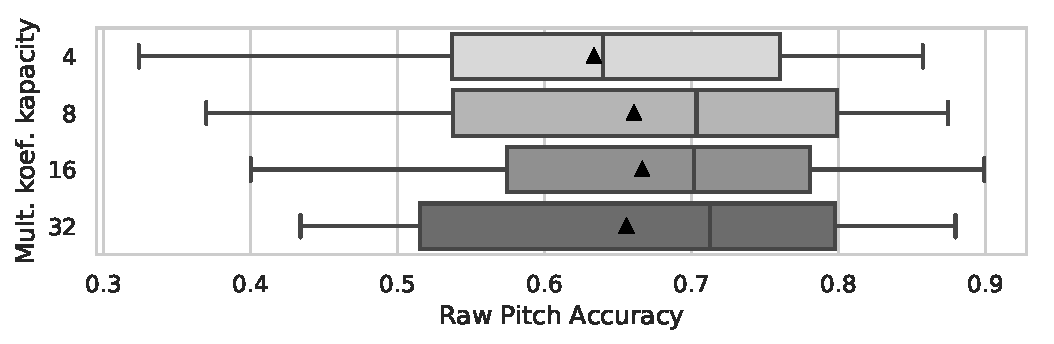
\includegraphics[scale=0.6]{../img/figures/crepe_kapacita_grey}
\caption{Výsledky experimentu s nezměněnou architekturou CREPE spuštěnou pro extrakci melodie.}
\label{obr:crepe_capacity_experiment}
\end{figure}

V tabulce \ref{tab:crepe_capacity_experiment} a na obrázku \ref{obr:crepe_capacity_experiment} uvádíme výsledky tohoto experimentu. Z validačních výsledků po $200\,000$ iteracích (přibližně 6 epoch) vidíme, že se výsledek modelů CREPE 8x a CREPE 16x liší řádově o desetiny procentních bodů. Přitom model s větší kapacitou se trénuje o 35\% delší dobu. Proto pro většinu následujících srovnávání zvolíme architektury s multiplikačním koeficientem 8, modely s dobrými výsledky případně přetrénujeme s vyšší kapacitou.

\subsection{Vliv rozlišení diskretizace výšky noty}\label{sec:crepe_diskretizace}

\begin{figure}[h]\centering
    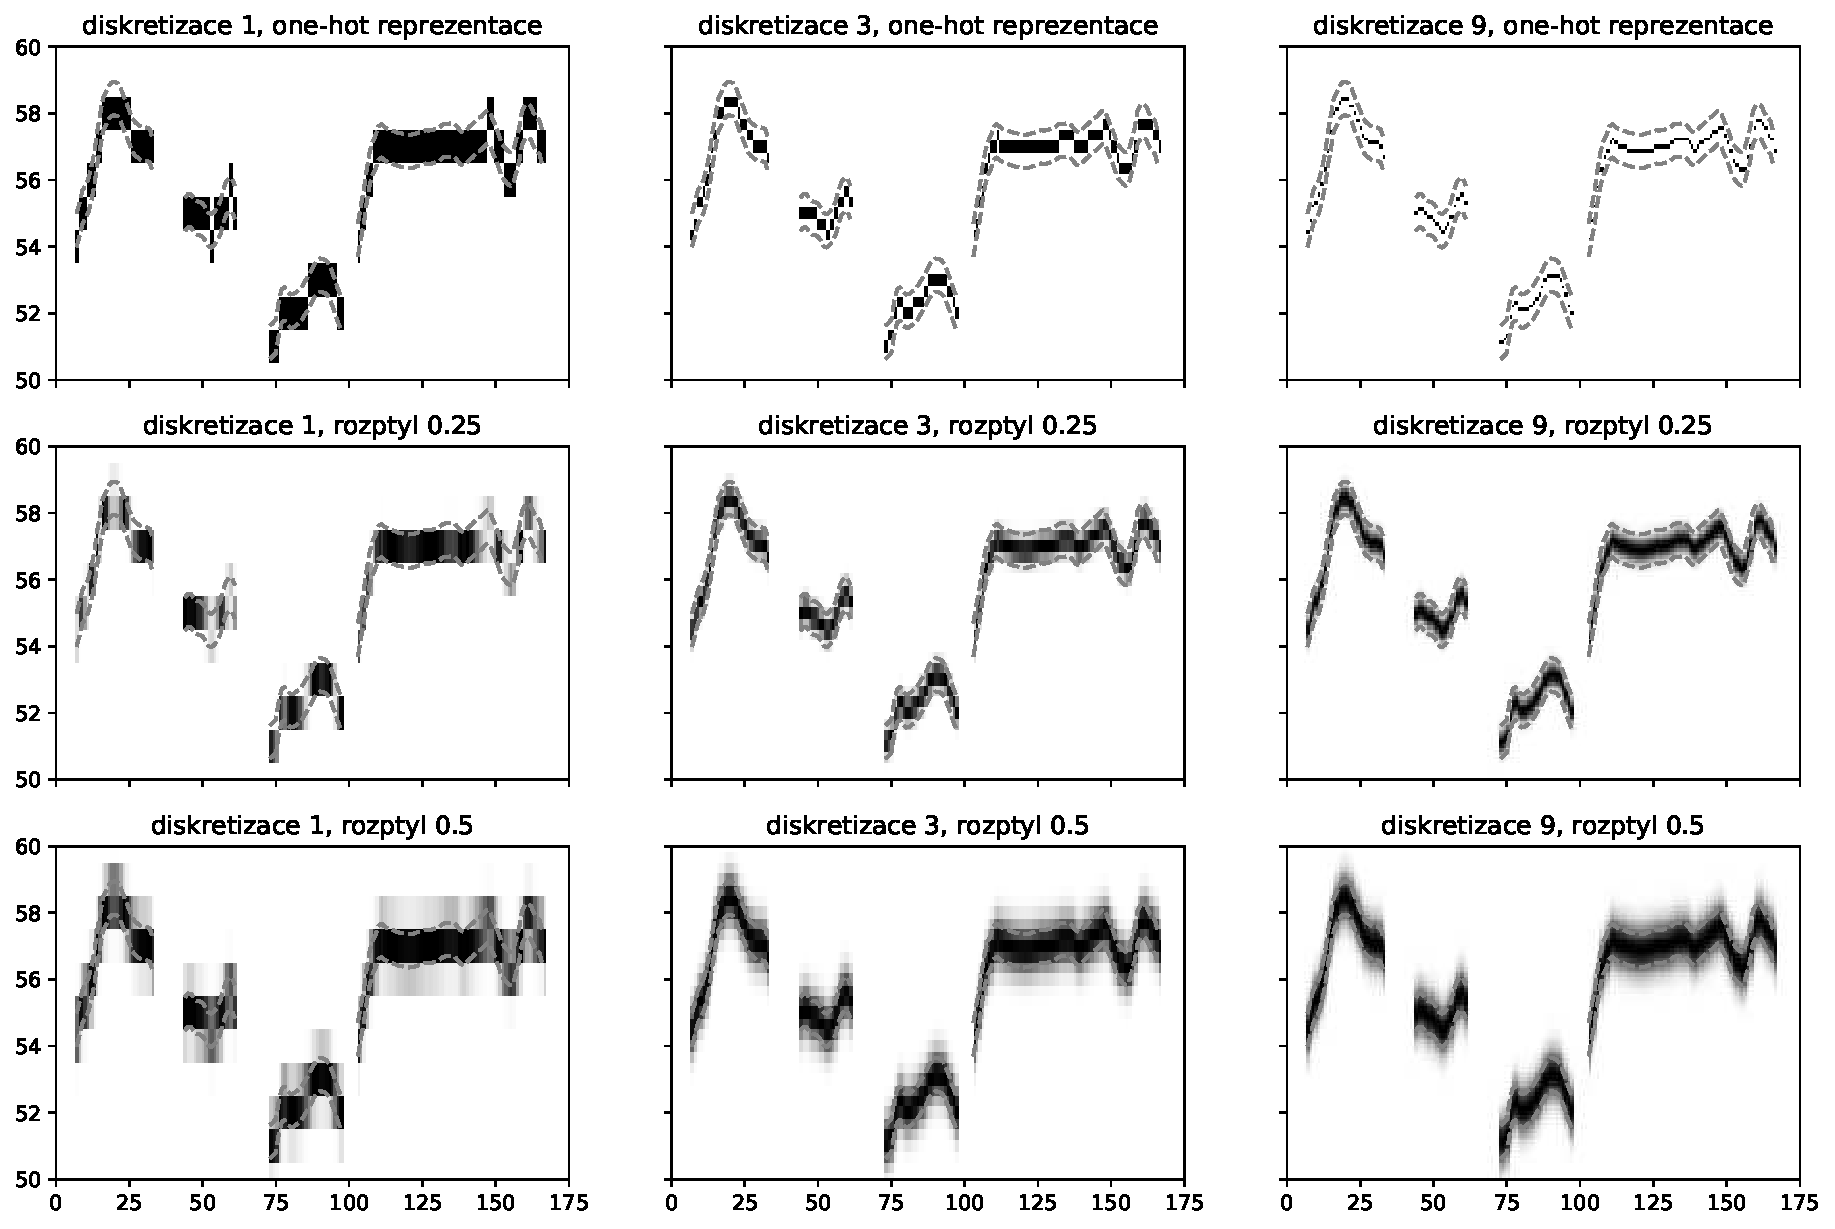
\includegraphics[width=\textwidth,height=\textheight,keepaspectratio]{../img/reprezentace_vstupu_grey}
\caption{Ukázky cílové reprezentace použité pro učení modelů. Pruhovaná linka značí dolní a horní hranici korektního odhadu výšky melodie.}\label{obr:reprezentace_vstupu}
\end{figure}

Otestujeme nastavení granularity výstupního vektoru. V článku \cite{Kim2018} se totiž důvod volby pěti frekvencí na půltón nediskutuje. Intuitivně by však mělo vyšší rozlišení spíše pomáhat, důvodem je, že nástroje a zejména lidský hlas se často při hraní odchylují od přesných, definovaných frekvencí hraných not a vyšší rozlišení tyto odchylky může lépe zachytit. Ve výsledku by pak síť s jemnějším výstupem měla dělat méně chyb, u kterých se skutečná a výstupní hodnota liší o jeden půltón. Na obrázku \ref{obr:reprezentace_vstupu} pro lepší představu uvádíme příklad cílových reprezentací s různým nastavením rozlišení diskretizace.

\begin{table}[h!]

\centering
    \begin{tabular}{rrr}
    \toprule
    Jemnost diskretizace &   RPA &   RCA \\
    \midrule
                    1 & 0.612 & 0.711 \\
                    3 & 0.653 & 0.760 \\
                    5 & 0.666 & 0.771 \\
                    7 & 0.654 & 0.763 \\
                    9 & 0.658 & 0.760 \\
    \bottomrule
    \end{tabular}

\caption{Architektura CREPE s různou jemností diskretizace.}\label{tab:crepe_diskretizace}

\end{table}

\begin{figure}[h]\centering
    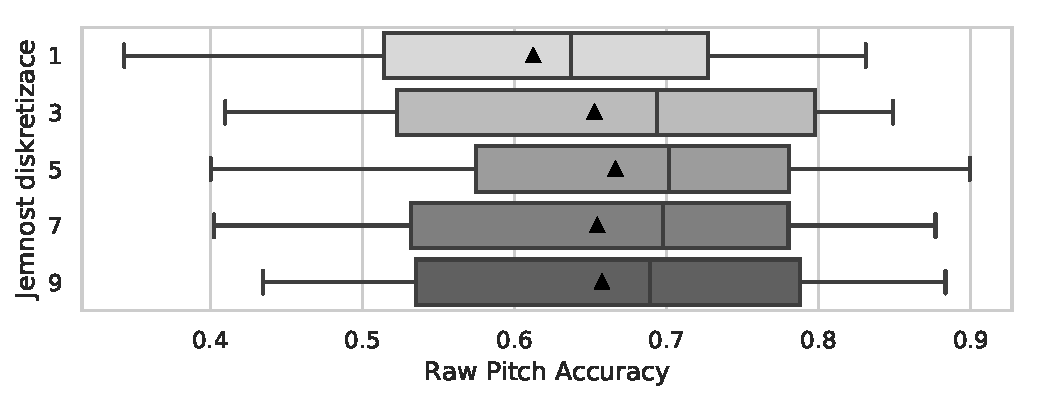
\includegraphics[scale=0.6]{../img/figures/crepe_diskretizace_grey}
\caption{Architektura CREPE s různou jemností diskretizace.}\label{obr:crepe_diskretizace}
\end{figure}

Jak můžeme pozorovat na výsledných hodnotách, jemná granularita výstupu zlepšuje přesnost sítě. Abychom ověřili domněnku, že vyšší rozlišení pomáhá zmenšit počet chyb o půltón, vytvoříme histogram vzdáleností cílového a odhadovaného tónu. V tomto histogramu by pak měl být zřetelný pokles v příslušných třídách. Podle histogramu se počet chyb o půltón mezi zkoumanými modely liší téměř o polovinu, zlepšení tohoto druhu chyb je tedy podstatné.

\begin{figure}[h]\centering
    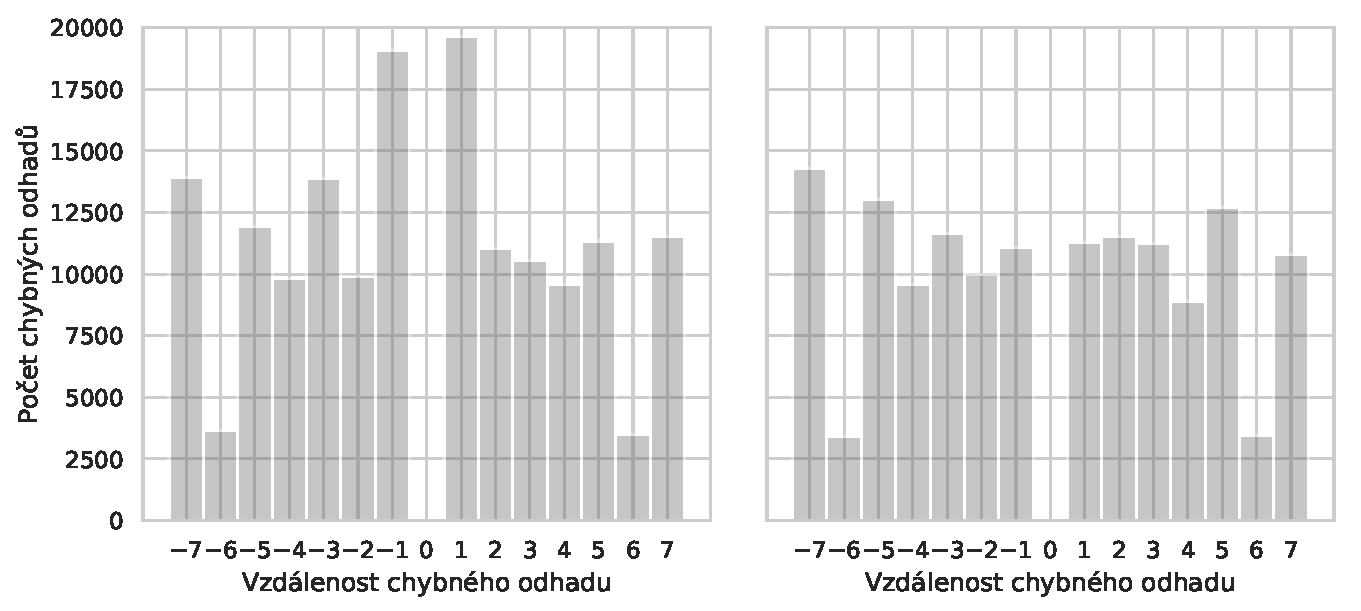
\includegraphics[scale=0.6]{../img/figures/crepe_diskretizace_hist_grey}
\caption{Histogramy vzdálenosti chybného odhadu, výstup prvního modelu má rozlišení 50 centů, výstup druhého 10 centů.}\label{obr:crepe_diskretizace}
\end{figure}

\subsection{Vliv rozptylu cílové pravděpodobnostní distribuce výšky noty}

Podle \cite{Bittner2017} pomáhá cílová distribuce s vyšším rozptylem snížit penalizaci sítě za téměř korektní odhady výšek tónů. Mimo to u dostupných dat často nejsou anotace naprosto perfektní, jisté rozostření hranice anotace tudíž pomáhá i v případě nepřesné cílové anotace, síť pak není tolik penalizována za svou případnou správnou odpověď. 

V článku se však nediskutuje, proč bylo zvoleno nastavení směrodatné odchylky na 20 centů. \cite{Kim2018} používá odchylku 25 centů a není na první pohled zřejmé, jaká je optimální hodnota. Příliš vysoký rozptyl způsobí, že síť bude tolerovat více chyb o půltón, příliš nízký rozptyl naopak penalizuje i za téměř správné odhady. Intuitivně se nejlepší nastavení pravděpodobně bude pohybovat kolem používaných 25 centů, jelikož to je hranice chybné klasifikace. Na obrázku \ref{obr:reprezentace_vstupu} pro lepší představu uvádíme příklad cílových reprezentací s různým nastavením rozptylu.

%  na druhou stranu optimální hodnota jistě bude závislá na nastavení rozlišení výstupního vektoru, jelikož nižší rozlišení bude jistě vyžadovat vyšší hodnotu rozptylu (v extrémním případě rozptylu blížícího se k nule a cílové frekvence mimo kvantizační hladiny by vzniklý cílový vektor nemusel obsahovat žádné ostré maximum).

% Poznamenám také technický detail, který je důležitý při samotné implementaci. Přestože jsem cílový výstup sítě zadefinoval jako diskrétní pravděpodobnostní rozdělení, při trénování je tento vektor hodnot pronásoben koeficientem tak, aby $\max(\mathbf{y}) = 1.0$ a tedy součet prvků vektoru není roven jedné (a o pravděpodobnostní rozdělení se doopravdy nejedná). Důvodem je použití aktivační funkce *sigmoid* u výstupní vrstvy, která nezaručuje výstup korektního rozdělení. Díky tomu se na výstupu může objevit různé množství stejně pravděpodobných kandidátů na melodii.

Testovaná síť má vstupní okno široké 4096 vzorků, používá multiplikátor kapacity 16x a vstup zpracovává 6 různě širokými konvolučními vrstvami (viz experiment \ref{exp:crepe_multirozliseni}).


\begin{table}[h!]
\centering
    \begin{tabular}{rrr}
    \toprule
    Rozptyl &   RPA &   RCA \\
    \midrule
    0.000 & 0.657 & 0.759 \\
    0.088 & 0.672 & 0.775 \\
    0.124 & 0.677 & 0.773 \\
    0.177 & 0.689 & 0.784 \\
    0.221 & 0.677 & 0.771 \\
    0.265 & 0.677 & 0.770 \\
    0.354 & 0.669 & 0.773 \\
    0.707 & 0.654 & 0.757 \\
    \bottomrule
    \end{tabular}

\caption{Architektura CREPE, vliv rozptylu cílové distribuce.}\label{tab:crepe_diskretizace}
\end{table}

\begin{figure}[h]\centering
    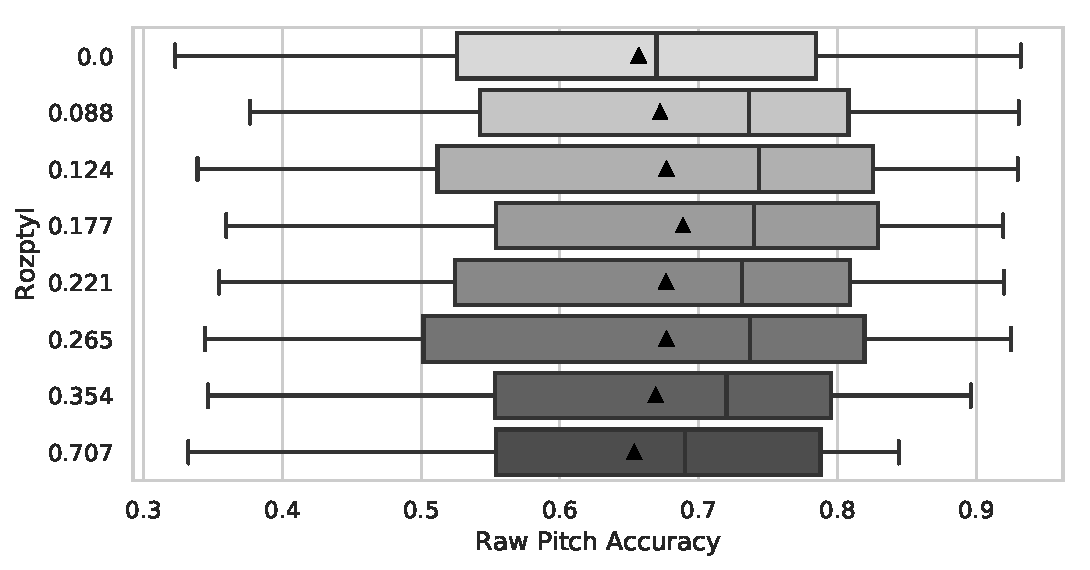
\includegraphics[scale=0.6]{../img/figures/crepe_rozptyl_grey}
\caption{Architektura CREPE, vliv rozptylu cílové distribuce.}\label{obr:crepe_diskretizace}
\end{figure}

Z experimentů vyplývá, že optimální směrodatná odchylka se pohybuje kolem hodnoty $0.177$, tedy níže než v porovnávaných pracích. Spolu s výsledky ze sekce \nameref{sec:crepe_diskretizace}, ve které ověřujeme nejlepší nastavení frekvenčního rozlišení, tedy docházíme k optimálnímu nastavení cílové reprezentace melodie, které budeme používat i v následujících experimentech se zbylými architekturami.

% ------
% - cílová distribuce doopravdy není distribuce
% - ty zvláštní testované směrod. odchylky jsou kvůli mé chybné implementaci rozostřování
% - zde můžu přidat obrázek, jak vypadají anotace
%     mám to rozpracované na: http://jirkabalhar.cz:6088/notebooks/bakalarka/algoritmy/ismir2017-deepsalience/deepsalience/out/io_comparison.ipynb#

\subsection{Vliv šířky vstupního okna}

Architektura CREPE byla navržena pro monopitch tracking, dá se předpokládat, že jelikož je v monofonních nahrávkách oproti polyfonním daleko méně (melodického) šumu, není pro určení výšky tónu potřeba větší kontext než použitých 1024 vzorků (při vzorkovací frekvenci 16kHz toto odpovídá 64 milisekundám audia). To ale nemusí platit pro složitější signály, kde by síť mohla z delšího kontextu těžit. Otestujeme tedy vliv většího vstupního okna na výslednou přesnost.


\begin{table}[h!]
\centering
    \begin{tabular}{rrr}
    \toprule
    Šířka vstupního okna &   RPA &   RCA \\
    \midrule
    512 (32 ms)   & 0.634 & 0.748 \\
    1024 (64 ms)  & 0.645 & 0.763 \\
    2048 (128 ms) & 0.648 & 0.760 \\
    4096 (256 ms) & 0.650 & 0.762 \\
    8192 (512 ms) & 0.675 & 0.775 \\
    \bottomrule
    \end{tabular}

\caption{Architektura CREPE, vliv šířky vstupního okna.}\label{tab:crepe_sirka}
\end{table}

\begin{figure}[h]\centering
    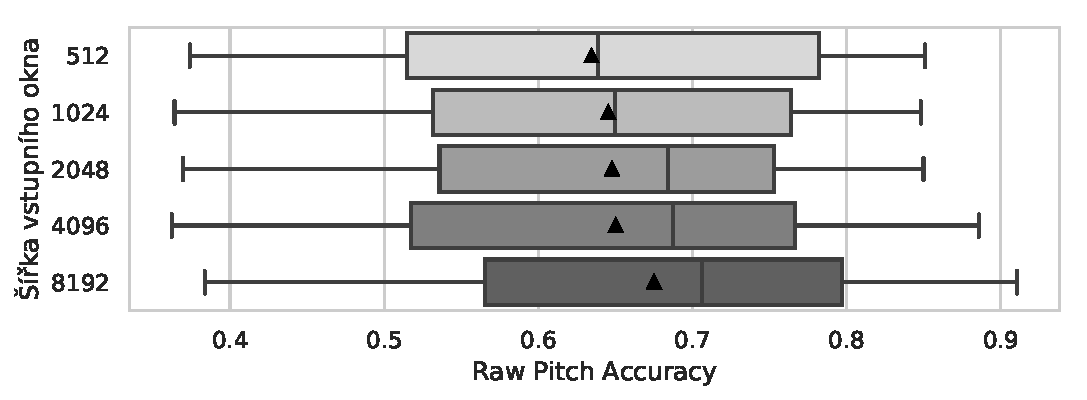
\includegraphics[scale=0.6]{../img/figures/crepe_sirka_grey}
\caption{Architektura CREPE, vliv rozptylu cílové distribuce.}\label{obr:crepe_sirka}
\end{figure}

Na obrázku \ref{tab:crepe_sirka} vidíme výsledky experimentu, mezi přesnostmi modelů s šířkou okna 1024 až 4096 vzorků nevidíme příliš veliké zlepšení, výsledek okna 8192 je však skokově lepší. Tento výrazný rozdíl spíše přičítáme jisté variabilitě výsledků při trénování neuronových sítí, není totiž zřejmé, jaká vlastnost vstupních dat by mohla způsobit tento skokový rozdíl.

% TODO: možná by to chtělo taky přetrénovat

% - širší okno se také hodí pro onsety a offsety

\subsection{Vliv násobného rozlišení první konvoluční vrstvy}\label{exp:crepe_multirozliseni}

Podle \cite{Kim2018} se přesnost CREPE snižuje s výškou tónu. Autoři si tuto skutečnost vysvětlují neschopností modelu generalizovat na barvy a výšky tónů neobsažených v trénovací množině, generalizaci by ale mohla pomoci také úprava modelu. Protože k rozpoznání vyšších frekvencí stačí méně vzorků než pro rozpoznání nižších, mohli bychom se pokusit upravit první konvoluční vrstvu sítě, která tento úkol rozpoznávání frekvencí ve vstupu zastává, a rozdělit ji na množinu různě širokých konvolucí, jejichž kanály následně sloučíme zpět do jednotné vrstvy. To by mohlo mít za následek, že rozpoznávání vysokých tónů budou zastávat užší konvoluce a jejich kernel bude jednodušší a obecnější, než když tuto funkci zastávají zbytečně široké kernely, u kterých je možné, že ve svých vahách obsahují redundantní informace.

První vrstvu s kernelem s 256 filtry (tj. počet filtrů první vrstvy s multiplikátorem 8x, viz první experiment) jsme rozdělili na více různě širokých kernelů s menším počtem filtrů, tak aby kapacita sítě zůstala přibližně stejná a sítě byly porovnatelné. Experiment jsme provedli na síti se vstupním oknem 2048 vzorků a multiplikátorem kapacity 8.

\begin{table}[h!]
\centering
    \begin{tabular}{lrrrrrrrrr}
    \toprule
    Šířka vrstev & 512 & 256 & 128 & 64 & 32 & 16 & 8  & 4  & Počet parametrů  \\
    Počet vrstev & {} & {} & {} & {} & {} & {} & {}  & {}  & {}  \\
    \midrule
    1                   & 256 &     &     &    &    &    &    &    & 2098880 \\
    2                   & 128 & 128 &     &    &    &    &    &    & 2066112 \\
    3                   & 85  & 85  & 85  &    &    &    &    &    & 2041918 \\
    4                   & 64  & 64  & 64  & 64 &    &    &    &    & 2029248 \\
    5                   & 51  & 51  & 51  & 51 & 51 &    &    &    & 2016350 \\
    6                   & 42  & 42  & 42  & 42 & 42 & 42 &    &    & 2001944 \\
    7                   & 36  & 36  & 36  & 36 & 36 & 36 & 36 &    & 1996184 \\
    8                   & 32  & 32  & 32  & 32 & 32 & 32 & 32 & 32 & 2000448 \\
    \bottomrule
    \end{tabular}
\caption{Počet filtrů prvních vrstev multirezoluční vstupní konvoluční vrstvy v architektuře CREPE.}\label{tab:crepe_velikosti_multirozliseni}
\end{table}

\begin{table}[h!]
\centering
    \begin{tabular}{rrr}
    \toprule
    Počet konvolučních vrstev &   RPA &   RCA \\
    \midrule
                            1 & 0.669 & 0.779 \\
                            2 & 0.669 & 0.773 \\
                            3 & 0.672 & 0.773 \\
                            4 & 0.674 & 0.778 \\
                            5 & 0.686 & 0.781 \\
                            6 & 0.678 & 0.780 \\
                            7 & 0.677 & 0.779 \\
                            8 & 0.680 & 0.778 \\
    \bottomrule
    \end{tabular}
\caption{Architektura CREPE, vliv multirezoluční vstupní konvoluční vrstvy.}\label{tab:crepe_multirozliseni}
\end{table}

\begin{figure}[h!]\centering
    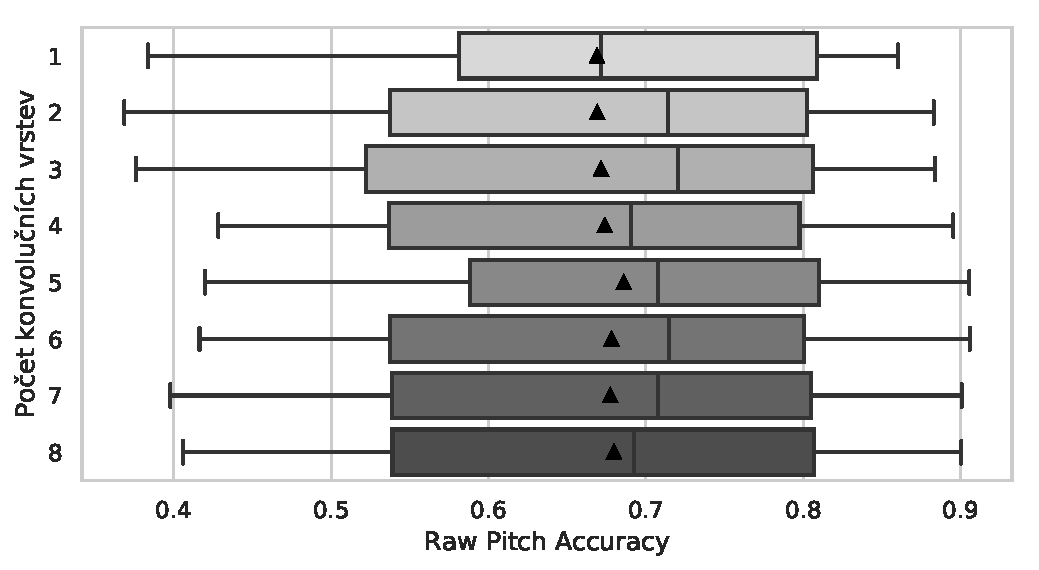
\includegraphics[scale=0.6]{../img/figures/crepe_multirozliseni_grey}
\caption{Architektura CREPE, vliv multirezoluční vstupní konvoluční vrstvy.}\label{obr:crepe_multirozliseni}
\end{figure}

Zlepšení výsledků se pohybuje v řádu desetin procentních bodů, nejvíce patrné je v případě pěti různě širokých konvolučních vrstev, kde dosahuje $1.3$ procentního bodu. Analýzou výsledků přesnosti podle výšky noty se mi nepodařilo prokázat domněnku, že by konvoluce s více rozlišeními pomáhala u odhadu not vyšších frekvencí. Její přínos je malý a projevuje se na většině frekvenčních pásem.

% \subsection{Shrnutí experimentů provedených s architekturou CREPE}

% \textcolor{red}{napsat shrnutí}

\section{Architektura WaveNet}\label{sec:wavenet}

Generativní model WaveNet popsaný týmem \cite{Oord2016} je architektura navržená pro generování zvukového signálu. Autoři však v článku zmiňují, že se architekturu pokusili využít i pro převod mluvené řeči na text (dataset TIMIT), a podařilo se jim dosáhnout výsledků srovnatelných se state-of-the-art. Architektura spočívá ve vrstvení dilatovaných konvolucí s rozšiřujícím se rozsahem. Díky exponenciálně rostoucím dilatacím se také exponenciálně zvětšuje receptivní pole jednotlivých konvolučních vrstev. Díky této vlastnosti pak například stačí pro pokrytí 1024 vzorků vstupu pouze 9 vrstev s šířkou kernelu 2 a dilatacemi 1,2,4,8 ... 512. Pokud bychom stejného receptivního pole chtěli dosáhnout pomocí obvyklých konvolucí počet potřebných vrstev by byl lineární vzhledem k šířce pole. Vrstvení konvolucí je porovnáno na obrázcích \ref{obr:wavenet_conv} a \ref{obr:wavenet_dilated}. Síť tedy velmi snadno pokryje široký kontext, což je vlastnost, která je pro zpracování zvukového signálu užitečná.

\begin{figure}[h!]\centering
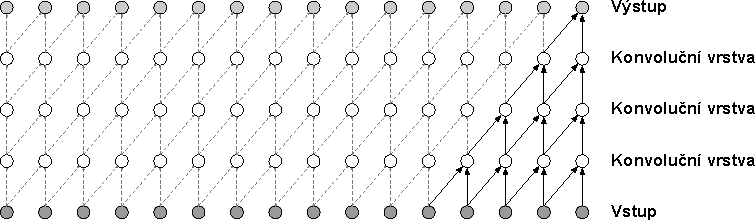
\includegraphics[scale=0.7]{../img/wavenet_konvoluce_grey}
\caption{Vrstvení obyčejných konvolucí s lineárně rozšiřovaným dosahem, obrázek převzat z \cite{Oord2016}.}
\label{obr:wavenet_conv}
\end{figure}

\begin{figure}[h!]\centering
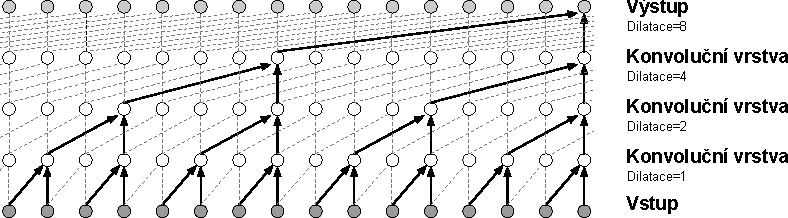
\includegraphics[scale=0.7]{../img/wavenet_dilatace_konvoluce_grey}
\caption{Vrstvení dilatovaných konvolucí s exponenciálně rozšiřovaným dosahem, obrázek převzat z \cite{Oord2016}.}
\label{obr:wavenet_dilated}
\end{figure}

Síť se pro Music Information Retrieval úlohy od svého zveřejnění příliš neuchytila. Její použití se v oblasti hudby se omezuje na generativní úlohy (\cite{Hawthorne2018a}, \cite{Yang2017}, \cite{Engel2017} a další), případně pro source-separation \citep{Stoller2018}. Jediný publikovaný pokus s použitím architektury WaveNet pro příbuznou úlohu kompletního automatického přepisu podnikli \cite{Martak2018} s použitím datasetu MusicNet. Jejich model však netestovali na standardních evaluačních datasetech ze soutěže MIREX, tudíž není zřejmé, jakých výsledků v porovnání s existujícími metodami autoři dosáhli.

V dalších sekcích se pokusíme nejprve spustit model \cite{Martak2018} na melodická data. Následně se pokoušíme tento výchozí výsledek zlepšit pomocí úpravy architektury WaveNet. Upravujeme celkovou kapacitu sítě pomocí nastavení počtu filtrů v dilatačních blocích. Dále pak měníme šířku kontextu, který je síti pro odhad jednoho bodu výšky tónu k dispozici, pomocí nastavení počtu dilatačních vrstev, bloků a velikosti šířky kernelů dilatací. Prozkoumáme také předzpracování vstupu do dilatačních bloků a způsob zpracování jejich výstupu.

\begin{figure}[h]\centering
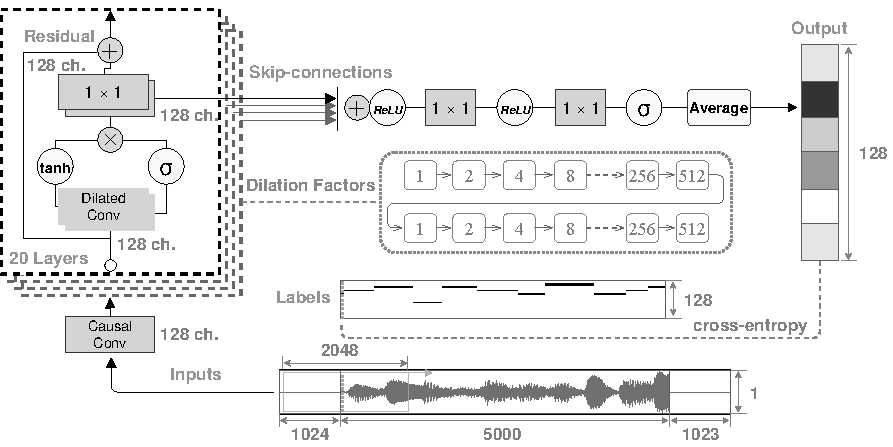
\includegraphics[width=\textwidth,height=\textheight,keepaspectratio]{../img/wavenet_arch_grey}
\caption{Architektura WaveNet upravená pro kompletní přepis skladeb, upraveno na základě \cite{Martak2018}.}
\label{obr:wavenet_arch}
\end{figure}

\subsection{Baseline na základě \cite{Martak2018}}

Pro extrakci melodie využijeme jako výchozí model upravenou architekturu od \cite{Martak2018}, jejíž struktura je naznačena na obrázku \ref{obr:wavenet_arch}. Vstupem je okno velikosti 4894 vzorků audia převzorkovaného na $16\,\rm kHz$, toto okno nejprve zpracujeme standardní konvoluční vrstvou s šířkou kernelu 2 a 128 výstupními kanály, takto zpracovaný signál dále prochází dvěma bloky po desíti vrstvách, které obsahují dilatované konvoluce. Vrstvy obsahují dvě dilatované konvoluce, jednu s aktivací hyperbolickým tangens a jednu s aktivační funkcí sigmoid. Výstupy těchto konvolucí jsou po složkách vynásobeny, díky čemuž konvoluce s aktivací sigmoid funguje jako nastavitelná propust signálu (Gated activation unit, \cite{Oord2016a}), poté je výstup opět zpracován dvěmi konvolucemi, tentokrát se šířkou kernelu 1x1. Výstup první sečteme s původním vstupem celé vrstvy (jedná se o residuální propojení poprvé popsané v práci \cite{He2015}) a zpracujeme ho nadcházející vrstvou. Výstup druhé konvoluce (autoři tuto cestu nazývají \emph{skip propojení}) zařadíme mezi výstupy skip propojení všech ostatních vrstev.

Pro výpočet odhadů výšky tónu sečteme všechna skip propojení, tento součet zpracujeme dvěma konvolucemi, druhá z nich má na výstupu 128 kanálů zpracovaných sigmoidou, což odpovídá rozsahu odhadovaných not. Jelikož všechny popsané transformace zachovávají šířku vstupu, dostáváme po této konvoluci odhady výšek not pro každý vstupní vzorek zvuku, taková anotace je zbytečně podrobná, tudíž výsledné anotace podvzorkujeme pomocí pooling vrstvy počítající průměr hodnot.

Po $20\,000$ iteracích s velikostí dávky 20 a parametrem learning rate $0.001$ síť dosahuje na validačních datech přesnost odhadu tónu $0.583$ (RPA) a přesnost odhadu tónu nezávisle na oktávě $0.692$ (RCA). V porovnání s výsledky architektury CREPE jsou tyto výsledky výrazně nižší, krom toho učení sítě trvá velmi dlouho (14 minut na 1000 iterací), zejména kvůli topologické komplexitě modelu. Síť také v této konfiguraci vykazuje známky přeučení. Pokusíme se tedy zrychlit trénování a zabránit přeučení použitím pouze jednoho dilatačního bloku a snížením počtu filtrů dilatačních a skip propojení ze 128 na 16. Také snížíme velikost trénovací dávky na 8 pro další zrychlení učení. Nová síť obsahuje 10 vrstev s dilatacemi $(1, 2, 4, 8, \dots, 512)$, celkový počet trénovatelných parametrů se z $2\,009\,728$ snížil na $34\,736$. Tato síť dosahuje RPA $0.598$ a RCA $0.696$ po $100\,000$ iteracích při rychlosti trénování 30 sekund na 1000 iterací. Síť tedy dosahuje stejných výsledků ve výrazně kratším čase.

Z předchozích experimentů na architektuře CREPE víme, že jemnější výstupní reprezentace pomáhá snížit počet chyb o půltón, upravíme tedy síť tak, aby na jeden půltón připadalo 5 výstupních složek vektoru, zmenšíme výstupní frekvenční rozsah a hodnoty cílového vektoru změníme z ostré predikce konkrétního tónu na \uv{rozmlžený} gaussián se směrodatnou odchylkou $18\,\rm centů$ (pro podrobnější popis viz \ref{sec:crepe}). Síť po této úpravě dosahuje RPA 0.629 a RCA 0.731 po $100\,000$ iteracích. 

\begin{figure}[h]\centering
    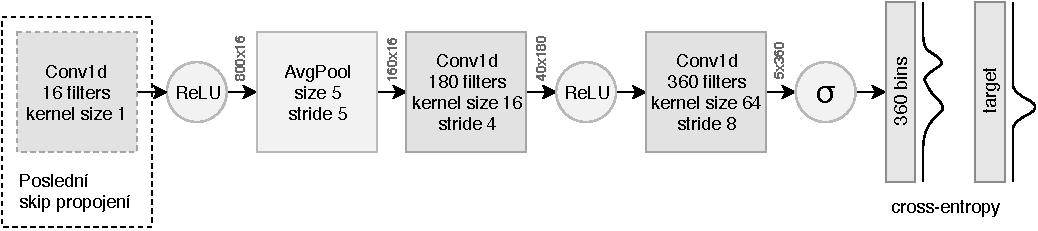
\includegraphics[scale=0.8]{../img/wavenet_lastlayer_grey}
    \caption{Úprava posledních vrstev WaveNet architektury.}\label{obr:wavenet_lastlayer}
\end{figure}

Předběžným hledáním výchozí architektury pro nadcházející sadu experimen\-tů jsme došli k následujícím úpravám. Dilatované konvoluce ve všech vrstvách mají šířku 3 místo 2, jejich vstup tedy závisí na všech okolních vzorcích, nikoli jen na předchozích, jak je naznačeno na obrázku \ref{obr:wavenet_dilated}. Dále jsme odstranili konvoluční vrstvu, která zpracovává vstup, ten je tedy přímo zpracován dilatačním blokem. Ze skip propojení se zpracovává pouze poslední, nedochází ke sčítání všech, což je úprava, kterou pro přepis řeči používají původní autoři článku WaveNet \cite{Oord2016}. Tento výstup je následně zpracován pooling vrstvou a dvěmi konvolucemi se skoky (stride), viz obrázek \ref{obr:wavenet_lastlayer}. Tato síť dosahuje RPA 0.655 a RCA 0.759 po $100\,000$ iteracích a je základem pro následující experimenty. 

\subsection{Vliv počtu filtrů dilatačních vrstev a skip propojení}

Jedním ze zásadních faktorů ovlivňujících kapacitu sítě je počet filtrů dilatačních vrstev a skip propojení. Tyto kanály nesou informaci o vzorku a jeho okolí, v závislosti na vrstvě dilatace. Výstup poslední vrstvy má tedy délku počtu vstupních vzorků 2848 a 16 kanálů. Každý výstupní vzorek nese informaci o svém okolí délky 2047. Podobně jako v případě architektury CREPE nalezneme vhodnou kapacitu sítě tak, aby nedocházelo k přeučení (overfitting) ani k nedoučení (underfitting) na trénovací množině.

\begin{table}[h!]
\centering
    \begin{tabular}{rrr}
    \toprule
    Počet kanálů &   RPA &   RCA \\
    \midrule
            4 & 0.609 & 0.714 \\
            8 & 0.628 & 0.739 \\
            16 & 0.655 & 0.759 \\
            24 & 0.665 & 0.764 \\
            32 & 0.671 & 0.771 \\
            40 & 0.667 & 0.766 \\
            48 & 0.667 & 0.764 \\
    \bottomrule
    \end{tabular}

\caption{Architektura WaveNet, vliv počtu filtrů dilatačních vrstev a skip propojení.}\label{tab:wavenet_dil_skip_channels}
\end{table}

\begin{figure}[h]\centering
    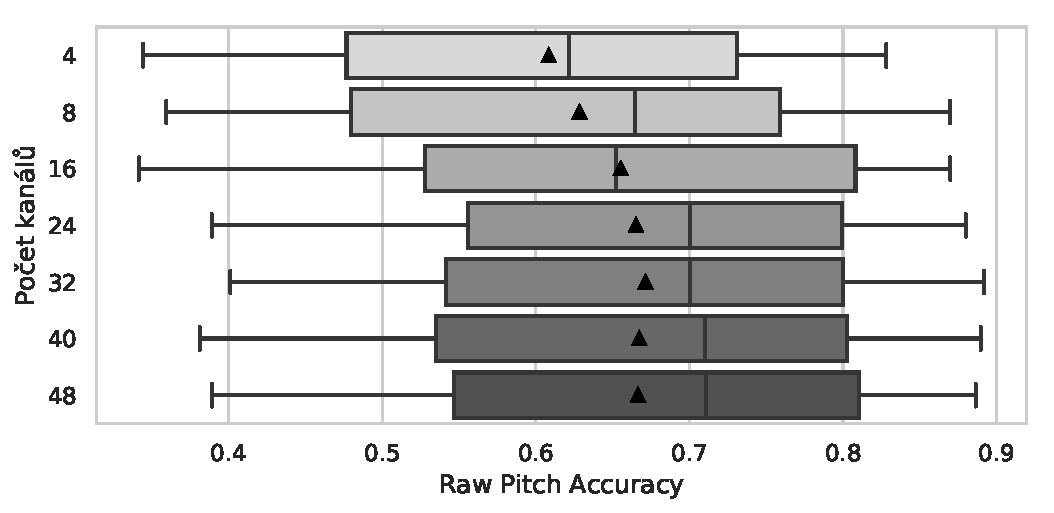
\includegraphics[scale=0.6]{../img/figures/wavenet_dil_skip_channels_grey}
\caption{Architektura WaveNet, vliv počtu filtrů dilatačních vrstev a skip propojení.}\label{obr:wavenet_dil_skip_channels}
\end{figure}

Na základě výsledků volíme pro další experimenty nastavení 16 filtrů pro dilatované konvoluce a skip propojení. Při nastavení 24 a více filtrů dosažená přesnost sítě stagnuje, 16 filtrů je kompromisem z hlediska rychlosti trénování.

\subsection{Systematické prohledávání počtu dilatačních vrstev a bloků}

Velikost zpracovávaného kontextu lze v architektuře WaveNet ovlivnit třemi různými hyperparametry. Jde o počet vrstev v bloku $n_{\mathrm{layers}}$, počet dilatačních bloků poskládaných nad sebou $n_{\mathrm{stacks}}$ a šířka kernelu dilatací $n_{\mathrm{width}}$. Přesně lze dosah vypočítat jako 

    $$\mathrm{receptive\_field} = (n_{\mathrm{width}}-1)\cdot(\sum_d^{n_{\mathrm{layers}}}{2^{(d-1)}})\cdot n_{\mathrm{stacks}}+1$$

Dosud jsme testovali sítě s jedním blokem o deseti vrstvách s dilatacemi $(1,2,4,8,16,\dots,512)$ s šířkou konvolucí 3, její dosah je tedy 2047 vzorků. Systematickým prohledáváním prozkoumáme vliv delšího kontextu měněného pomocí $n_{\mathrm{layers}}$ a $n_{\mathrm{stacks}}$. Při vyhodnocování experimentu je nutné vzít v úvahu, že přidání nové vrstvy, případně celého nového bloku, zároveň zvyšuje kapacitu modelu, což také ovlivňuje výslednou přesnost modelu. Šířky kontextu a kapacity jsou uvedené v tabulce \ref{tab:wavenet_dilation_width_numbers}.

V architektuře modelu jsme pro tento experiment provedli změnu ve zpracování skip propojení. V této sadě se nebere poslední skip propojení, nýbrž všechna se spojí v ose kanálů a slouží jako vstup pro následující pooling vrstvu a konvoluci. Z toho důvodu má model mnohem více parametrů, na druhou stranu je zajištěno, že poslední vrstvy mohou využít informace ze všech skip spojení k odhadu výšek. Na základě srovnání tréninkové a validační ztrátové funkce však modely nevykazují známky přeučení.

\begin{table}[h!]
\centering
    \begin{tabular}{lrrrrr}
    \toprule
    Max. dilatace & 64 & 128 & 256 & 512 & 1024 \\
    Počet bloků   & {} & {}  & {}  & {}  & {}  \\
    \midrule
    1 (dosah) & 255  & 511  & 1023 & 2047 & 4095 \\
    1 (kapacita) & $4\,483\,644$  & $4\,531\,836$ & $4\,580\,028$ & $4\,628\,220$ & $4\,676\,412$ \\
    2 (dosah) & 509  & 1021 & 2045 & 4093 & 8189 \\
    2 (kapacita) & $4\,820\,988$  & $4\,917\,372$ & $5\,013\,756$ & $5\,110\,140$ & $5\,206\,524$ \\
    3 (dosah) & 763  & 1531 & 3067 & 6139 & $12\,283$ \\
    3 (kapacita) & $5\,158\,332$  & $5\,302\,908$ & $5\,447\,484$ & $5\,592\,060$ & $5\,736\,636$ \\
    4 (dosah) & 1017 & 2041 & 4089 & 8185 & --- \\
    4 (kapacita) & $5\,495\,676$  & $5\,688\,444$ & $5\,881\,212$ & $6\,073\,980$ & --- \\
    \bottomrule
    \end{tabular}
\caption{Architektura WaveNet, dosah a kapacita v závislosti na dilatačních počtu vrstev a bloků.}\label{tab:wavenet_dilation_width_numbers}
\end{table}

\begin{figure}[h]\centering
    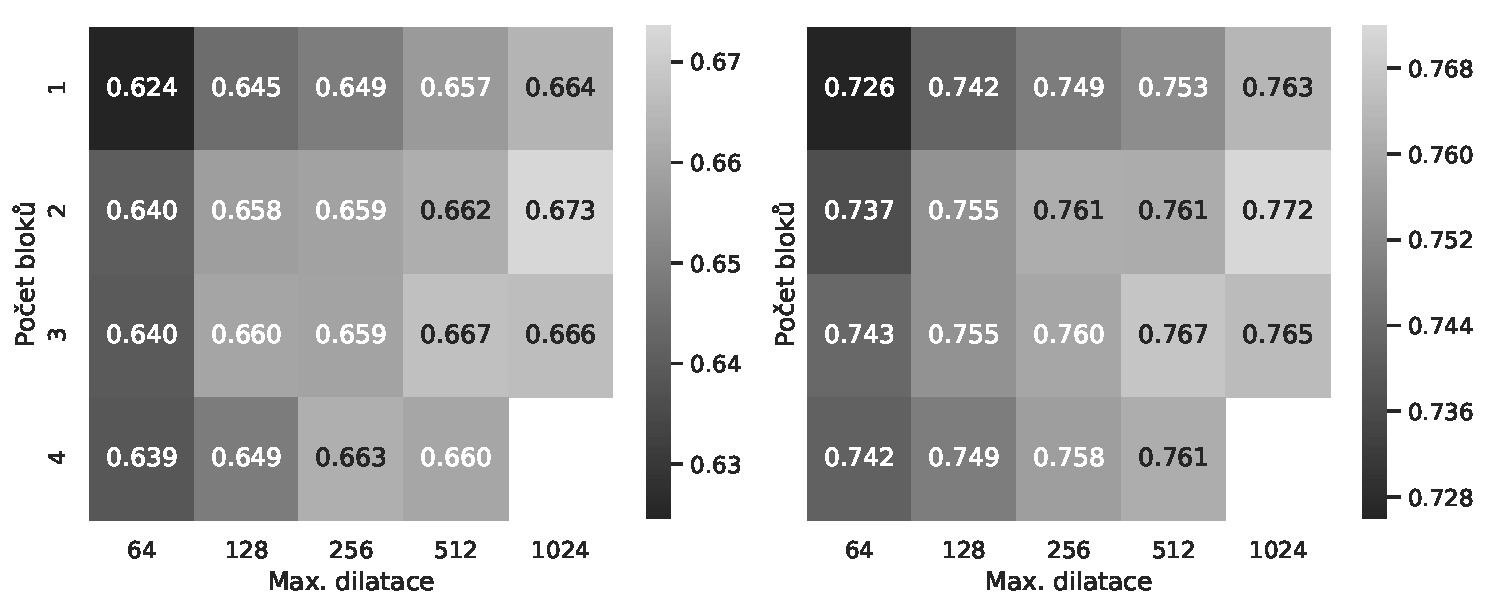
\includegraphics[scale=0.5]{../img/figures/wavenet_stacks_gridsearch_grey}
\caption{Architektura WaveNet, systematické prohledávání počtu dilatačních vrstev a bloků, vlevo hodnoty RPA, vpravo RCA.}\label{obr:wavenet_stacks_gridsearch}
\end{figure}

Na základě obrázku \ref{obr:wavenet_stacks_gridsearch} lze dojít k pozorování, že přidávání počtu vrstev zvyšuje výslednou přesnost víceméně vždy, to neplatí o počtu bloků, u kterých se zdá, že nejvhodnější počet je 2. Pokud se zaměříme na srovnání výsledků s podobným dosahem, zdá se že výsledky jsou poměrně podobné, zejména pro širší dosahy, pro kratší se zdá lepší využít spíše více vrstev než více bloků. 

\subsection{Vliv velikosti šířky kernelu dilatací}

Jiným způsobem, jak zvýšit velikost zpracovávaného kontextu, je volba velikosti šířky kernelu dilatací $n_{\mathrm{width}}$. Provedeme čtyři experimenty s různou šířkou. Šířka 2 je zvolena v původním článku z toho důvodu, že konvoluce se tím stávají \uv{kauzální} --- jejich výstup závisí pouze na vzorcích před nimi (viz obrázky \ref{obr:wavenet_conv}, \ref{obr:wavenet_dilated}). To je výhodné pro generativní úlohy, u kterých chceme, aby hodnota nového generovaného vzorku v audio signálu nezávisela na budoucích, zatím neexistujících vzorkách. U klasifikačních úloh takto omezeni nejsme, tudíž můžeme s nastavením experimentovat. 

\begin{table}[h!]
\centering
    \begin{tabular}{rrr}
    \toprule
    Šířka kernelu dilatací &   RPA &   RCA \\
    \midrule
                        2 & 0.649 & 0.754 \\
                        3 & 0.648 & 0.755 \\
                        4 & 0.656 & 0.759 \\
                        5 & 0.645 & 0.756 \\
    \bottomrule
    \end{tabular}
\caption{Architektura WaveNet, vliv velikosti šířky kernelu dilatací.}\label{tab:wavenet_dilation_width}
\end{table}

\begin{figure}[h]\centering
    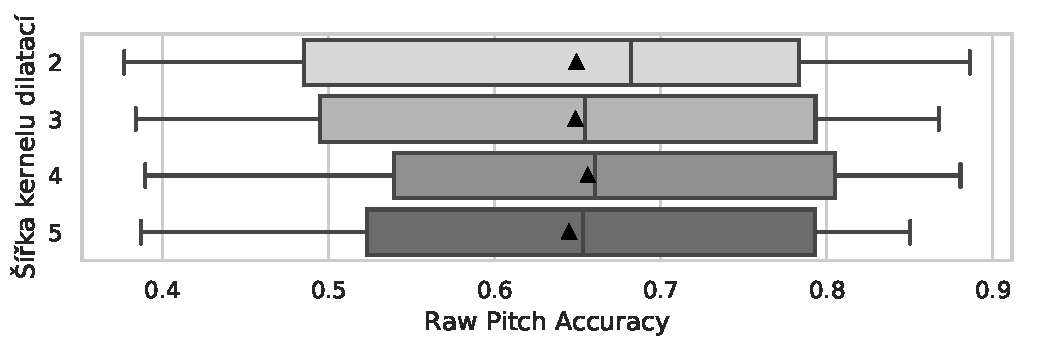
\includegraphics[scale=0.6]{../img/figures/wavenet_dilation_width_grey}
\caption{Architektura WaveNet, vliv velikosti šířky kernelu dilatací.}\label{obr:wavenet_dilation_width}
\end{figure}

Z tabulky \ref{tab:wavenet_dilation_width} a grafu \ref{obr:wavenet_dilation_width} vyplývá, že tato síť při změnách šířky kernelu dilatace svou výslednou přesnost na validačních datech nemění.

\subsection{Vliv výstupní transformace skip propojení}

Volba transformace skip propojení se v článku týmu \cite{Oord2016} nediskutuje, \cite{Martak2018} také přejímají součet všech skip výstupů. Vyzkoušíme proto dvě další možnosti práce se skip propojeními - výběr posledního skip propojení a dále spojení všech skip propojení do mnohakanálového výstupu. V případě výběru posledního propojení či součtu jde o transformace, které lze vyjádřit jako speciální případ konvoluce nad spojenými skip propojeními. Dalo by se tedy říct, že výběr a součet jsou v tomto případě speciálními případy spojených výstupů. Testovaná možnost výběr poslední vrstvy skip propojení naopak přináší jinou výhodu - pro výpočet výsledku sítě nejsou potřeba zbylá skip propojení, což urychluje trénování.

\begin{table}[h!]
\centering
    \begin{tabular}{lrr}
    \toprule
    Transf. skip vrstev &   RPA &   RCA \\
    \midrule
            Konkatenace & 0.654 & 0.754 \\
            Poslední & 0.651 & 0.754 \\
                Součet & 0.646 & 0.753 \\
    \bottomrule
    \end{tabular}

\caption{Architektura WaveNet, vliv výstupní transformace skip propojení.}\label{tab:wavenet_skip_reduction}
\end{table}

\begin{figure}[h]\centering
    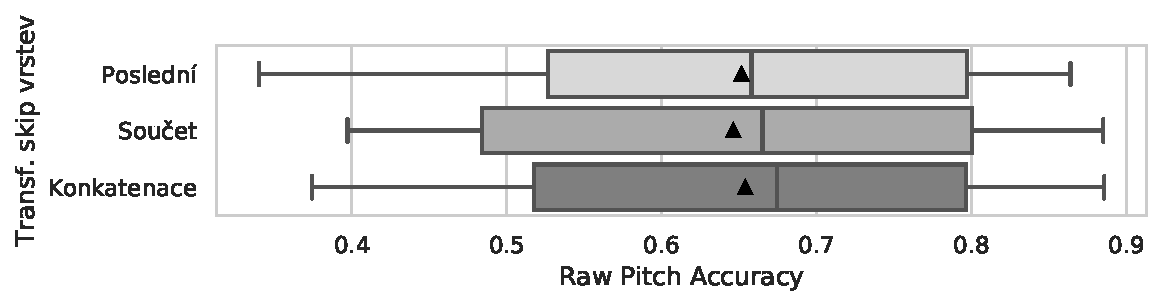
\includegraphics[scale=0.6  ]{../img/figures/wavenet_skip_reduction_grey}
\caption{Architektura WaveNet, vliv výstupní transformace skip propojení.}\label{obr:wavenet_skip_reduction}
\end{figure}

Všechny tři transformace vedou ke stejné přesnosti. Síť tedy netěží z větších možností práce s dřívejšími vrstvami a nejdůležitejší informace se objevují až na vrchu bloků dilatovaných konvolucí.

\subsection{Vliv velikosti první konvoluce}

Tým \cite{Oord2016} používá pro předzpracování zvukového signálu před vstupem do dilatovaných bloků obvyklou konvoluci, nespecifikuje však její šířku. Veřejná implementace architektury WaveNet pracuje s šířkou 32.\footnote{\url{https://github.com/ibab/tensorflow-wavenet/blob/master/wavenet_params.json}} \cite{Martak2018} používají šířku 2, čímž fakticky jen duplikují první dilatační vrstvu. První vrstva může sloužit jako banka filtrů, podobně jako první vrstva v architektuře CREPE. Aby však pro tento účel mohla fungovat plnohodnotně, musela by být široká minimálně 512 vzorků, aby mohla zachytit periodu i té nejnižší frekvence ve výstupním rozsahu. Pomocí sady experimentů se pokusíme zjistit, zda má první konvoluční vrstva pozitivní vliv na výslednou přesnost.


\begin{table}[h!]
\centering
    \begin{tabular}{rrr}
    \toprule
    Velikost první vrstvy &   RPA &   RCA \\
    \midrule
                        0 & 0.648 & 0.755 \\
                        8 & 0.663 & 0.762 \\
                    16 & 0.661 & 0.765 \\
                    32 & 0.654 & 0.754 \\
                    64 & 0.643 & 0.756 \\
                    256 & 0.609 & 0.735 \\
                    1024 & 0.601 & 0.734 \\
    \bottomrule
    \end{tabular}
\caption{Architektura WaveNet, vliv velikosti první konvoluce.}\label{tab:wavenet_first_layer}
\end{table}

\begin{figure}[h]\centering
    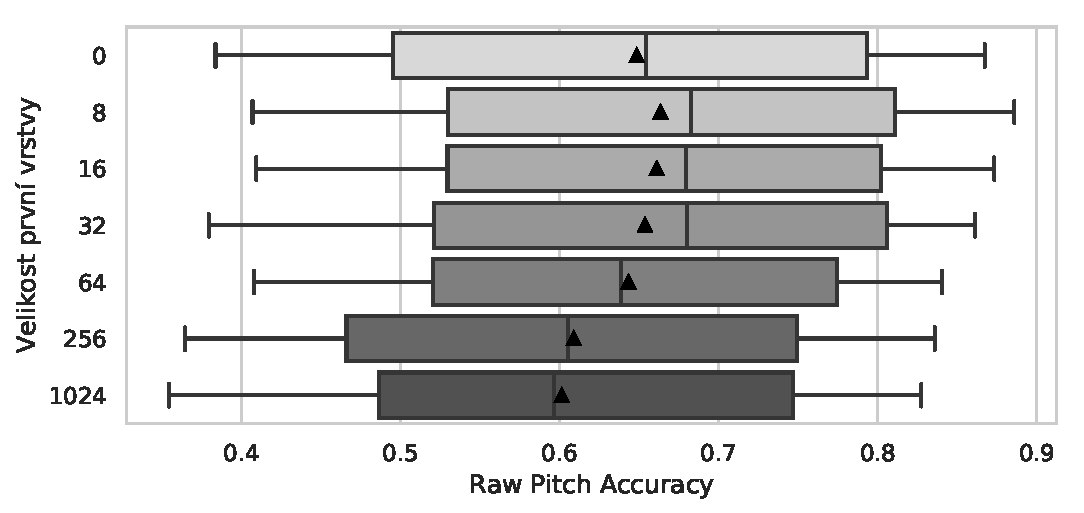
\includegraphics[scale=0.6]{../img/figures/wavenet_first_layer_grey}
\caption{Architektura WaveNet, vliv velikosti první konvoluce.}\label{obr:wavenet_first_layer}
\end{figure}

Sítě, které mají možnost využít první konvoluce jako banky filtrů, dosahují výrazně horší přesnosti, než sítě s menší konvolucí. Přeskočení tohoto předzpracování však také není nejlepším nastavením pro tuto architekturu. Vhodná šířka první konvoluce se pohybuje kolem 8 vstupních vzorků, do takové šířky se vejde jedna perioda signálu frekvence $2000\,\rm Hz$, jinými slovy vrstva jistě nemůže zastávat ani z části funkci banky filtrů. Mohla by však popisovat sklon křivky vstupních dat, ze kterých se v dalších vrstvách dilatovaných bloků složí již celý frekvenční popis vstupu.

% \textcolor{red}{vizualizace první vrstvy? Co tam vlastně může být, když pomáhá šestnácti samplová konvoluce?}
% \textcolor{red}{Zase by to tady chtělo nějaké shrnutí pokusů s WaveNetem — odkud kam jste se s ním dostal. Začlo se tím, že se použily triky nalezené na pokusech s CREPE, potom se dělaly ještě nějaké triky s WaveNet-specific choices}

% \subsection{Vliv návrhu posledních vrstev}

% \begin{table}[h!]
% \centering
% \caption{Architektura WaveNet, vliv návrhu posledních vrstev.}\label{tab:wavenet_output_transform}
% \end{table}

% \begin{figure}[h]\centering
%     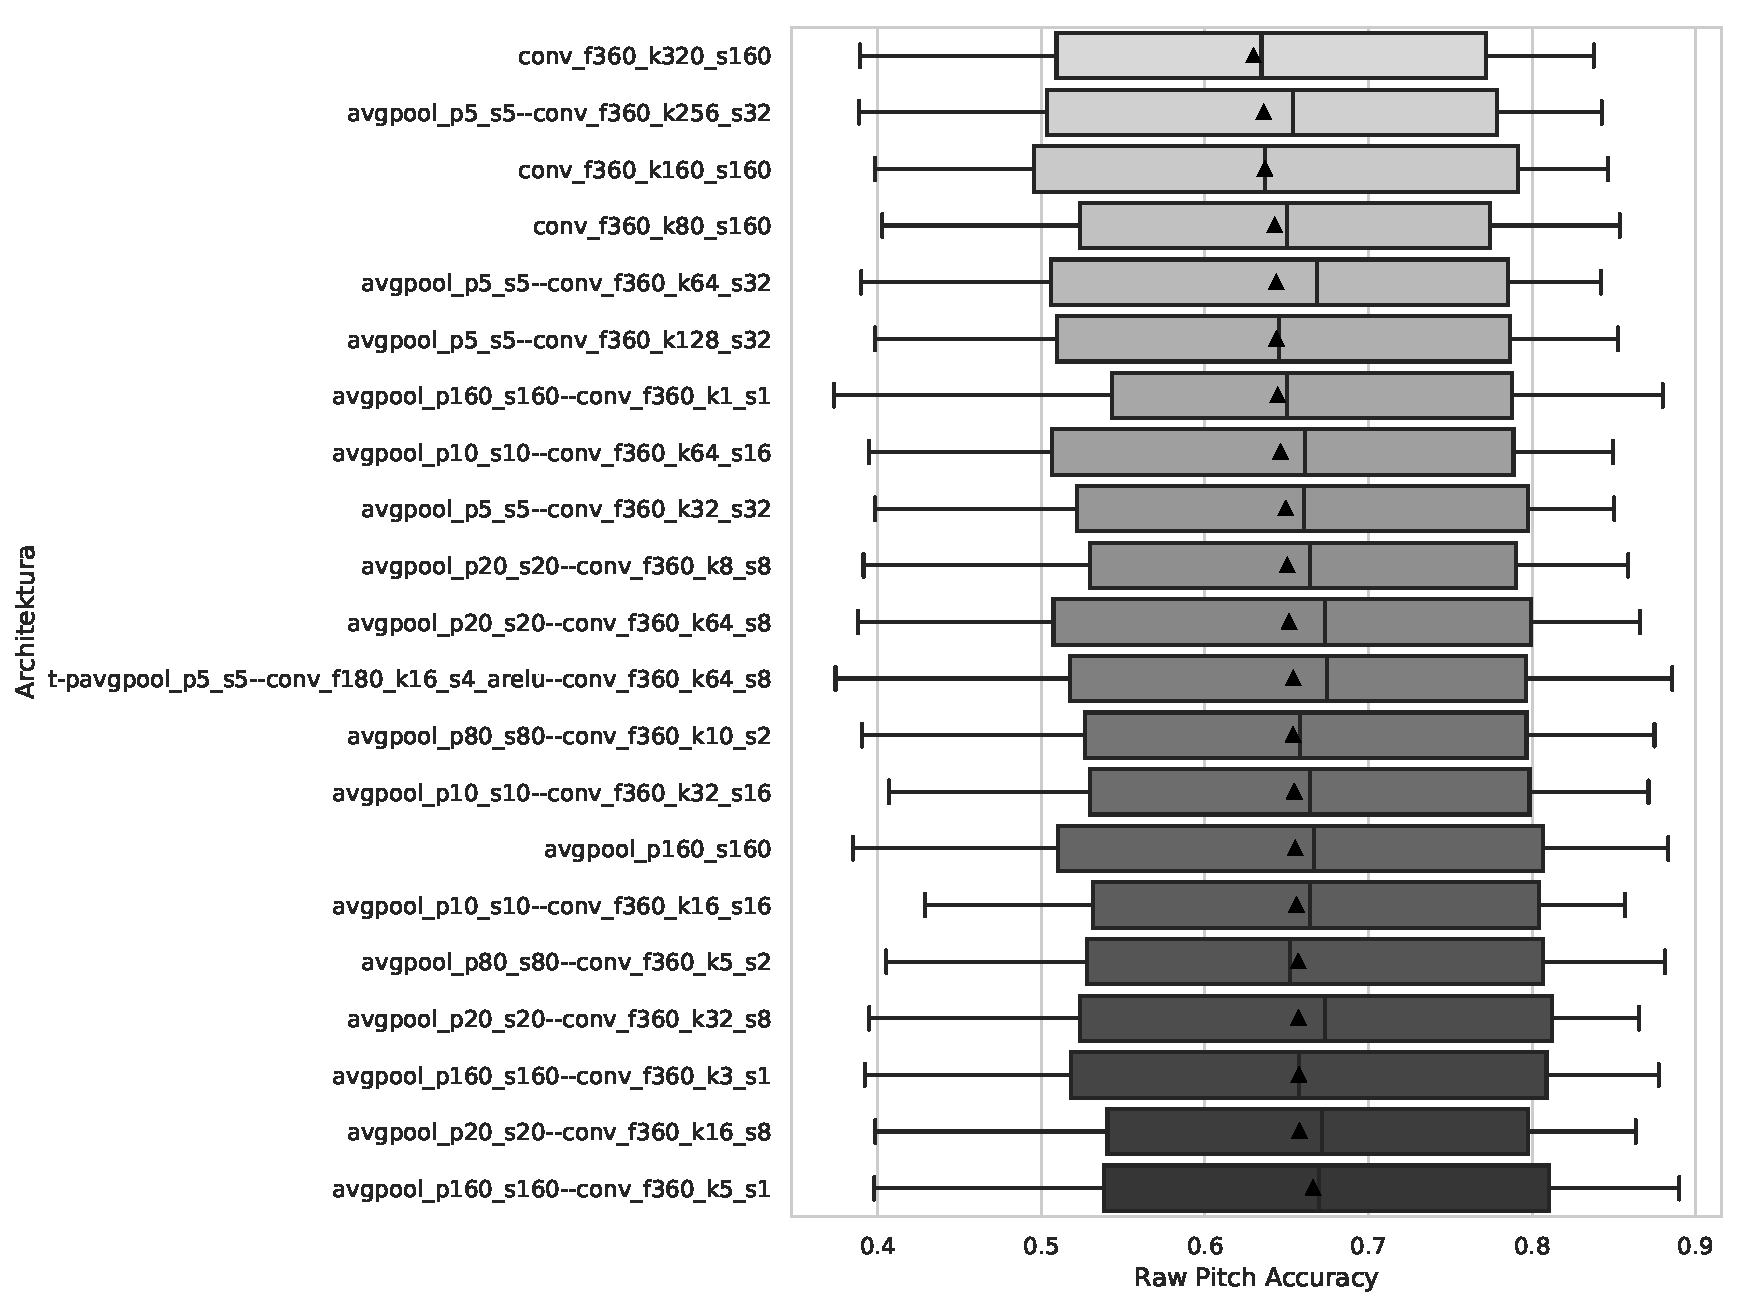
\includegraphics[scale=0.6]{../img/figures/wavenet_output_transform_grey}
% \caption{Architektura WaveNet, vliv návrhu posledních vrstev.}\label{obr:wavenet_output_transform}
% \end{figure}

\section{Architektura HCNN}

\begin{figure}[h]\centering
    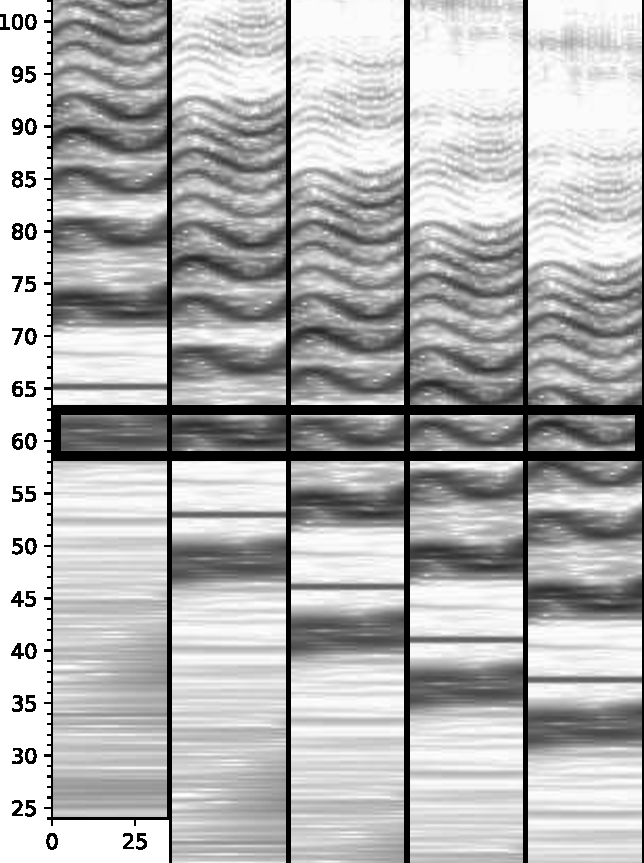
\includegraphics[scale=0.5]{../img/spectrograms_grey}
\caption{Znázornění harmonických závislostí na spektrogramu s logaritmickou osou frekvence.}\label{obr:hcqt}
\end{figure}

V práci prezentujeme také novou architekturu pro zpracování harmonicky strukturovaných zvukových signálů kterou nazýváme \emph{Harmonic Convolutional Neural Network}. Inspirujeme se prací \cite{Bittner2017}, která problém výpočtu salienční funkce zasazuje do rámce úlohy odstranění šumu v obrázku pomocí konvolučních sítí. Její architektura vstupní spektrogram zpracovává několika konvolučními vrstvami, výsledkem pak je nový spektrogram s odstraněným \uv{šumem hudebního doprovodu}. 

Dalším přínosem její práce je popis vstupní spektrální reprezentace HCQT. CQT spektrogramy mají logaritmickou osu frekvence, tato reprezentace má tu vlastnost, že dvě libovolné harmonické frekvence jednoho tónu mají na spektrogramu mezi sebou konstantní vzdálenost, nezávislou na fundamentální frekvenci. HCQT spočívá ve výpočtu několika CQT spektrogramů, jejichž frekvenční rozsahy jsou vzájemně posunuty právě o tyto konstatní vzdálenosti. Pokud pak tyto spektrogramy poskládáme za sebe v nové ose kolmé na osu frekvence a času, harmonické frekvence se překryjí (viz obrázek \ref{obr:hcqt}). Tento vícekanálový spektrogram pak může sloužit jako vstup pro konvoluční vrstvu, která má při výpočtu jedné frekvenční složky k dispozici také informace o souvisejících harmonických složkách.

Z této myšlenky úpravy vstupní reprezentace pro rozšiřování receptivního pole konvoluce na související harmonické složky vychází naše architektura HCNN. Síť je koncipována jako obvyklé vrstvení konvolučních vrstev, každému konvolučnímu bloku však předchází úprava vstupu takovým způsobem, aby do výpočtu nadcházející konvoluce byly zahrnuty i potenciální harmonické složky dané frekvence. Naše metoda tedy nepracuje pouze s výpočtem různých CQT spektrogramů na vstupu jako práce \cite{Bittner2017}, upravujeme totiž mezivýsledky všech vrstev v síti a naše transformace spočívá v pouhém posunutí, nikoli přepočítávání. Na obrázku \ref{obr:hcnn_harmonic_stacking} tuto úpravu vstupu znázorňujeme; výstup předchozí konvoluční vrstvy duplikujeme a vzájemně posuneme o pevně dané počty půltónů tak, aby harmonicky související složky byly umístěny \uv{nad sebou} v dimenzi kanálů. Následně výstupy v této dimenzi spojíme a chybějící složky doplníme nulami.

Tato úprava přináší dvě výhody. Jednak síť může využít relevantní harmonické informace v každé vrstvě a ne pouze na vstupu, což vede k lepší přesnosti modelů. Také ale můžeme díky harmonické transformaci velmi výrazně zmenšit samotné konvoluční vrstvy. Zatímco konvoluční vrstvy v architektuře \cite{Bittner2017} používají velké kernely (zejména pak ve frekveční ose) a na výstupu vrací velké množství kanálů, aby byly schopná zachytit vzdálené frekvenční závislosti, díky struktuře HCNN takto velké konvoluční vrstvy nejsou potřeba. Ve výsledku naše testované architektury obsahují řádově desetkrát méně parametrů a trénují se v rámci desítek až stovek minut.

\begin{figure}[h]\centering
    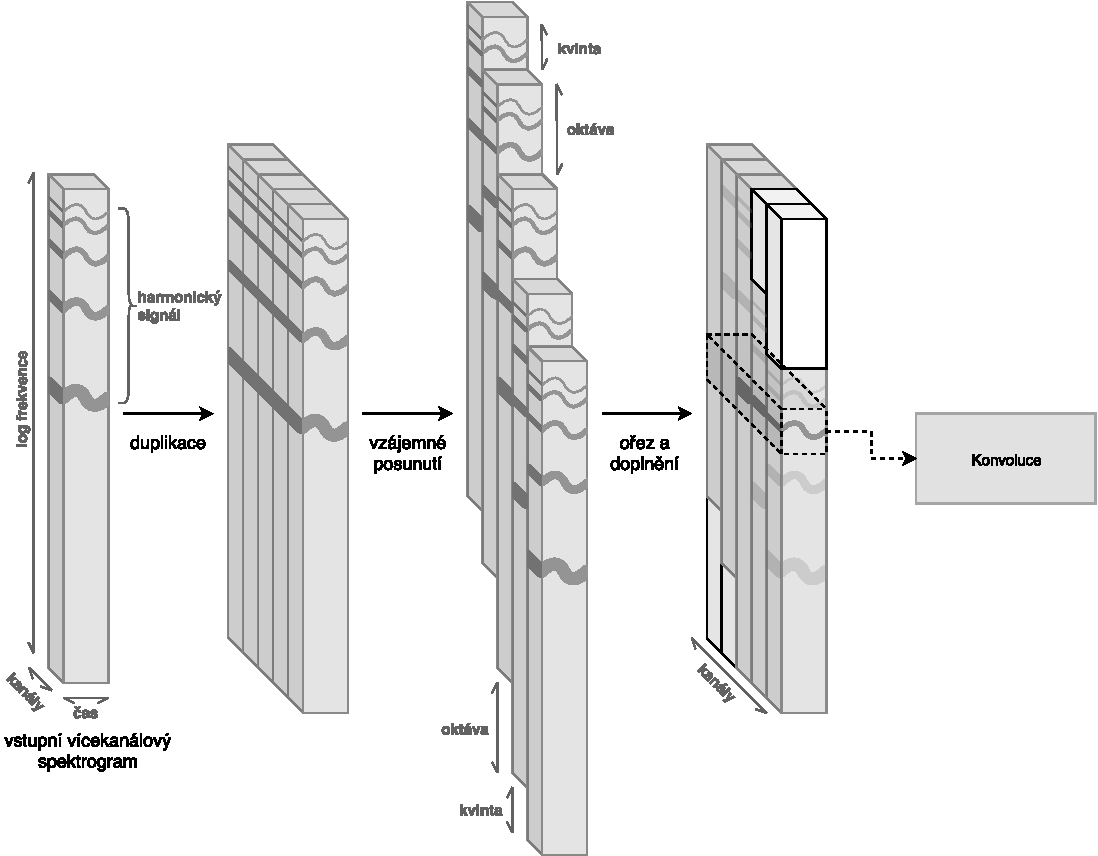
\includegraphics[width=\textwidth,height=\textheight,keepaspectratio]{../img/hcnn_harmonic_stacking_2_grey}
\caption{Diagram transformace vstupu konvoluční vrstvy pro zachycení harmonických souvislostí.}\label{obr:hcnn_harmonic_stacking}
\end{figure}

\begin{figure}[h]\centering
    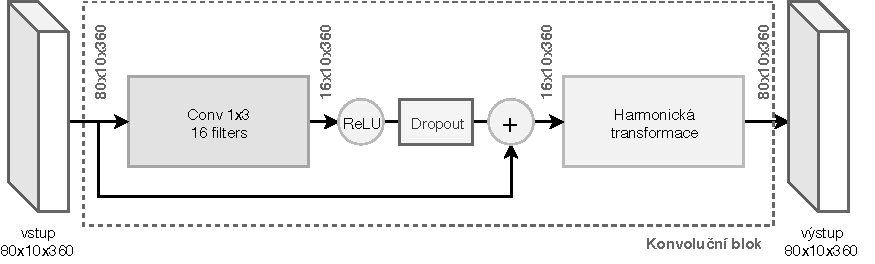
\includegraphics[width=\textwidth,height=\textheight,keepaspectratio]{../img/hcnn_layer_grey}
\caption{Diagram konvolučního bloku architektury HCNN.}\label{obr:hcnn_layer}
\end{figure}

\begin{figure}[h]\centering
    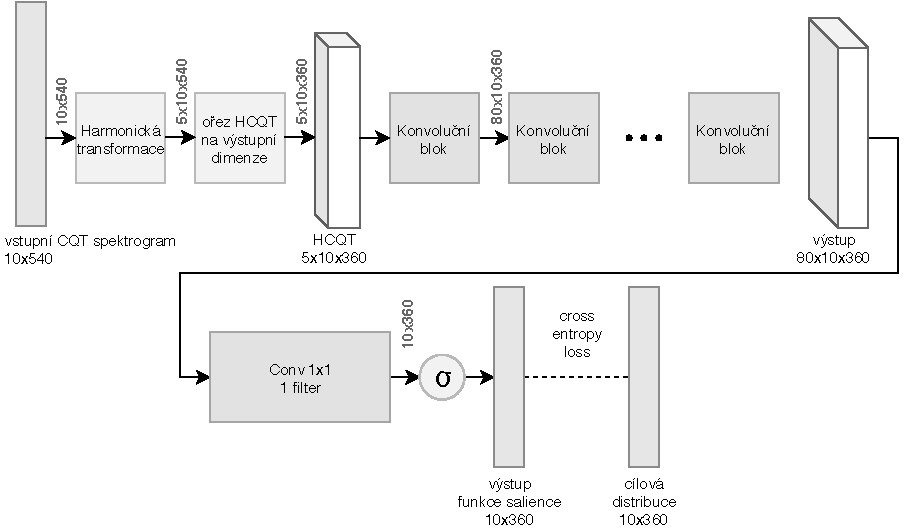
\includegraphics[width=\textwidth,height=\textheight,keepaspectratio]{../img/hcnn_arch_grey}
\caption{Diagram celkového propojení architektury HCNN.}\label{obr:hcnn_arch}
\end{figure}

Zbývající prvky architektury již čerpají ze zavedených postupů. Diagram \ref{obr:hcnn_layer} znázorňuje strukturu jednoho konvolučního bloku; po každé konvoluční vrstvě s aktivační funkcí ReLU následuje dropout vrstva a kolem konvoluce vedeme residuální propojení pro umožnění trénování hlubokých architektur. Celková architektura (obrázek \ref{obr:hcnn_arch}) pak spočívá v harmonické transformaci vstupní CQT (čímž efektivně vytvoříme reprezentaci odpovídající HCQT bez přepočítávání každého CQT zvlášť), aplikaci několika konvolučních bloků a aplikaci konvoluce 1x1 pro transformaci výstupu zpět na jeden dvoudimenzionání výstup.

Vstupní CQT počítáme z původních audio souborů se vzorkovací frekvencí $44\,100\,\rm Hz$, používáme implementaci algoritmu z balíku \texttt{librosa} a parametry transformace jsou: počáteční frekvence (\texttt{fmin}) = 32.7 (Tón C1), počet složek na oktávu (\texttt{bins\_per\_octave}) = 60 (vychází 5 složek na půltón, jako v předchozích sekcích), počet složek (\texttt{n\_bins}) = 540 (vychází na 9 oktáv, po první harmonické transformaci však spektrogram ořízneme na výšku 360, zbylé složky jsou přítomny, aby zaplnily chybějící hodnoty, které vzniknou při harmonických posunech), \texttt{hop\_size}=256 (tudíž jedno anotační okno MedleyDB odpovídá jednomu sloupci vstupního spektrogramu). Dále pak hodnoty vstupu převedeme na logaritmickou škálu dBFS (funkce \texttt{librosa.core.amplitude\_to\_db}). 

Cílový výstup počítáme v souladu s implementacemi v předchozích sekcích, tedy použijeme normální rozdělení se střední hodnotou rovnou výšce znějící melodie a rozptylem 18 centů.

V následujících experimentech nejprve prokážeme užitečnost aplikace harmonické transformace uvnitř sítí a nalezneme vhodnou hloubku a kapacitu modelů, dále prezentujeme jednu z limitací vstupní reprezentace práce \cite{Bittner2017} a pokusíme se navrhnout vlastní rozšíření vstupní reprezentace. V závěru se pokusíme rozšířit sítí zpracovávaný kontext a zběžně otestujeme i možnost použití augmentace vstupních spektrogramů.

\subsection{Harmonické transformace}

Abychom prokázali pozitivní vliv harmonické transformace, natrénujeme tři sady modelů. Jednu sadu bez jakýchkoliv transformací, sadu s transformací s posunutím o $\pm 12$ půltónů (zachycení druhé harmonické složky) a třetí sadu s posunutím o $\pm 12$ a o $\pm 19$ půltónů (zachycení druhé a třetí harmonické složky). Vstupem všech sítí bude HCQT (implementovaný efektivně pomocí harmonických posunů), aby byl posouzen vliv transformací uvnitř sítě, nikoli také na vstupu.

\begin{figure}[h!]\centering
    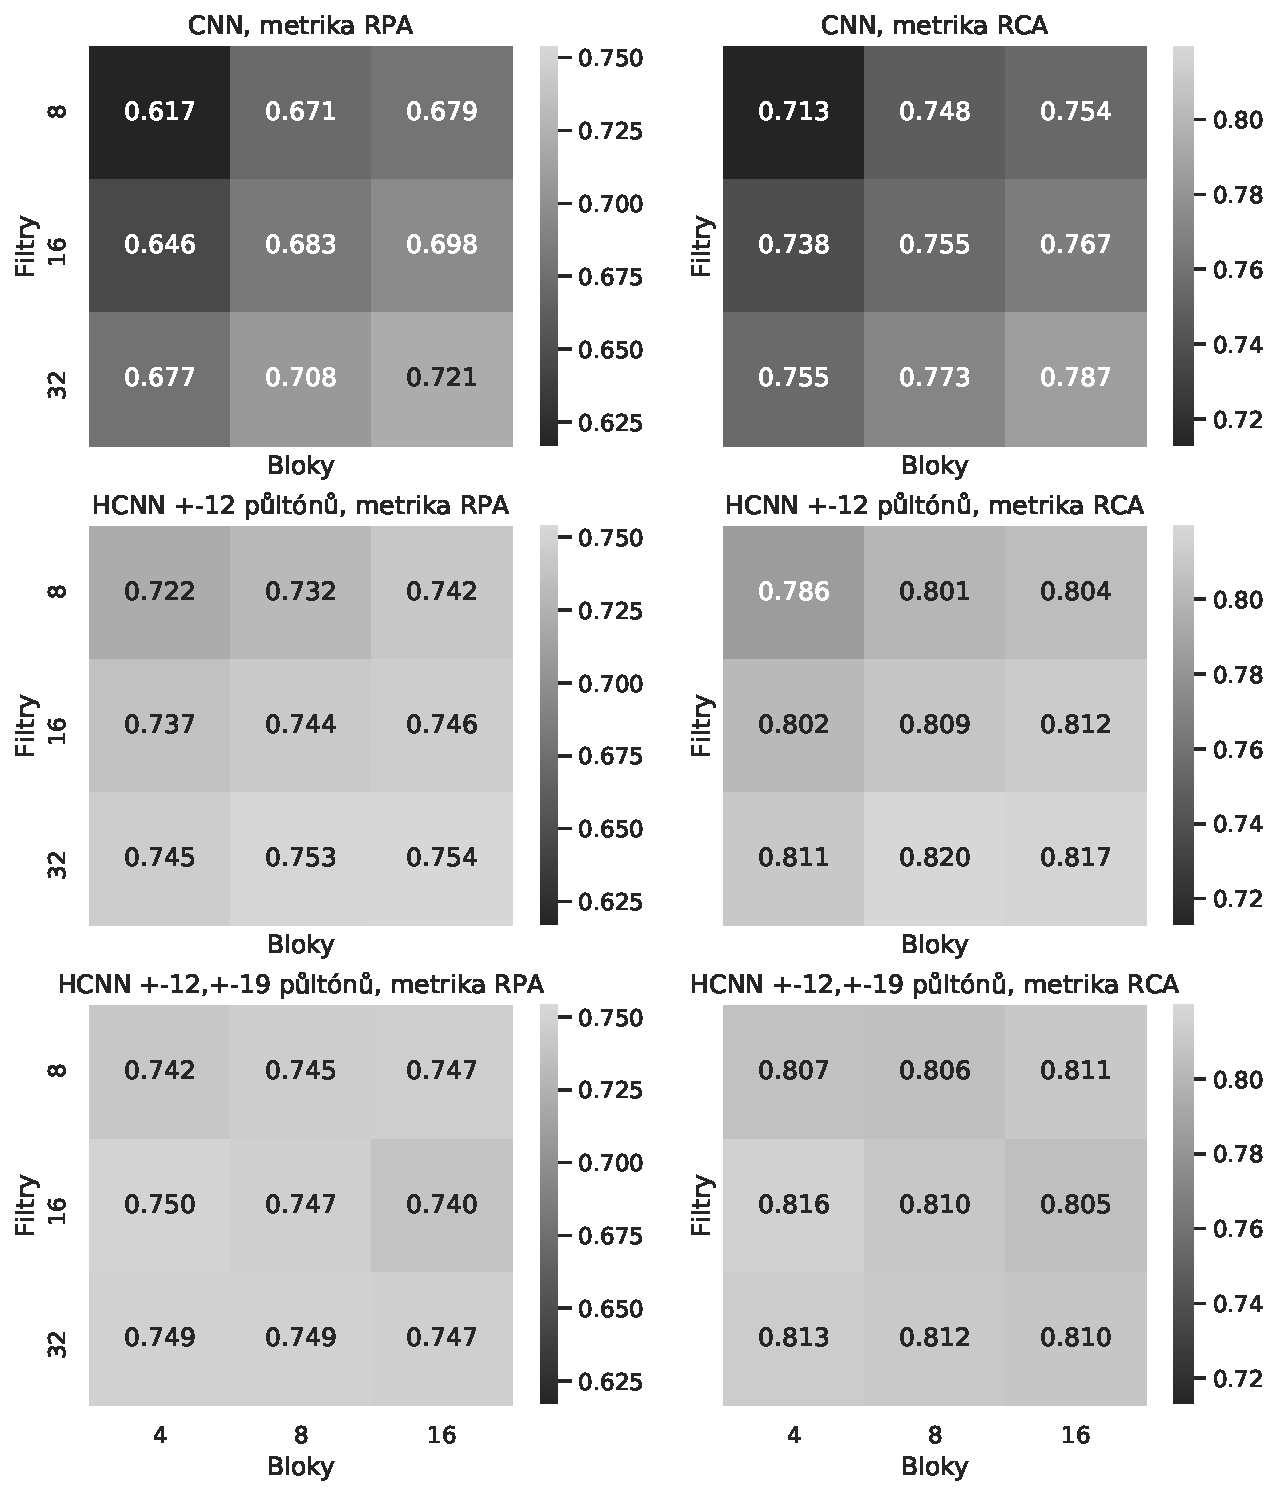
\includegraphics[scale=0.55]{../img/figures/spectrogram_harmonic_stacking_grey}
\caption{Architektura HCNN, Detekce melodie, vliv počáteční pooling vrstvy.}\label{obr:spectrogram_harmonic_stacking}
\end{figure}

Na základě porovnání všech kombinací počtů filtrů a bloků na obrázku \ref{obr:spectrogram_harmonic_stacking} je jisté, že použití harmonické transformace uvnitř konvolučních sítí pomáhá zvyšovat přesnost. U všech testovaných šířek a hloubek sítí došlo k několikaprocentnímu nárustu přesnosti přepisu. Ukazuje se, že k tomuto nárustu došlo přidáním pouze dvou posunutí --- posunutí o oktávu v ose frekvence nahoru a dolů. Přidáním další zachycené harmonické frekvence sice pomůžeme zvýšit přesnost modelů s menší kapacitou, modelům s vyšší kapacitou již úprava nepomáhá. 

\subsection{Parametr \texttt{hop\_size}}

Metoda \cite{Bittner2017} pracuje se spektrogramy CQT vypočítanými s velikostí skoku $\approx 11\,\rm ms$. Data MedleyDB, která v práci používáme, jsou však anotována s velikostí skoku $\approx 5.8\,\rm ms$. To znamená, že při trénování musíme anotace v trénovací množině MedleyDB podvzorkovat a podobně při vyhodnocování výsledků sítě musíme výstup převzorkovat zpět na původní časové rozlišení datasetu. V obou případech převzorkování můžeme ztratit informace, které se projeví v horší výsledné přesnosti. Je také otázkou, zda-li je nejlepší postup, pokud síť budeme trénovat na neoriginálních, převzorkovaných datech. Na druhou stranu výhodou většího skoku je větší receptivní pole konvoluce, kernel o šířce větší než 1 má na podvzorkovaných datech dvojnásobný dosah. Tento efekt lze nicméně napodobit nastavením dvojnásobné dilatace konvoluce. Na experimentech s kernely šířky 1 posoudíme dopad převzorkování bez této zmiňované výhody.

\begin{figure}[h]\centering
    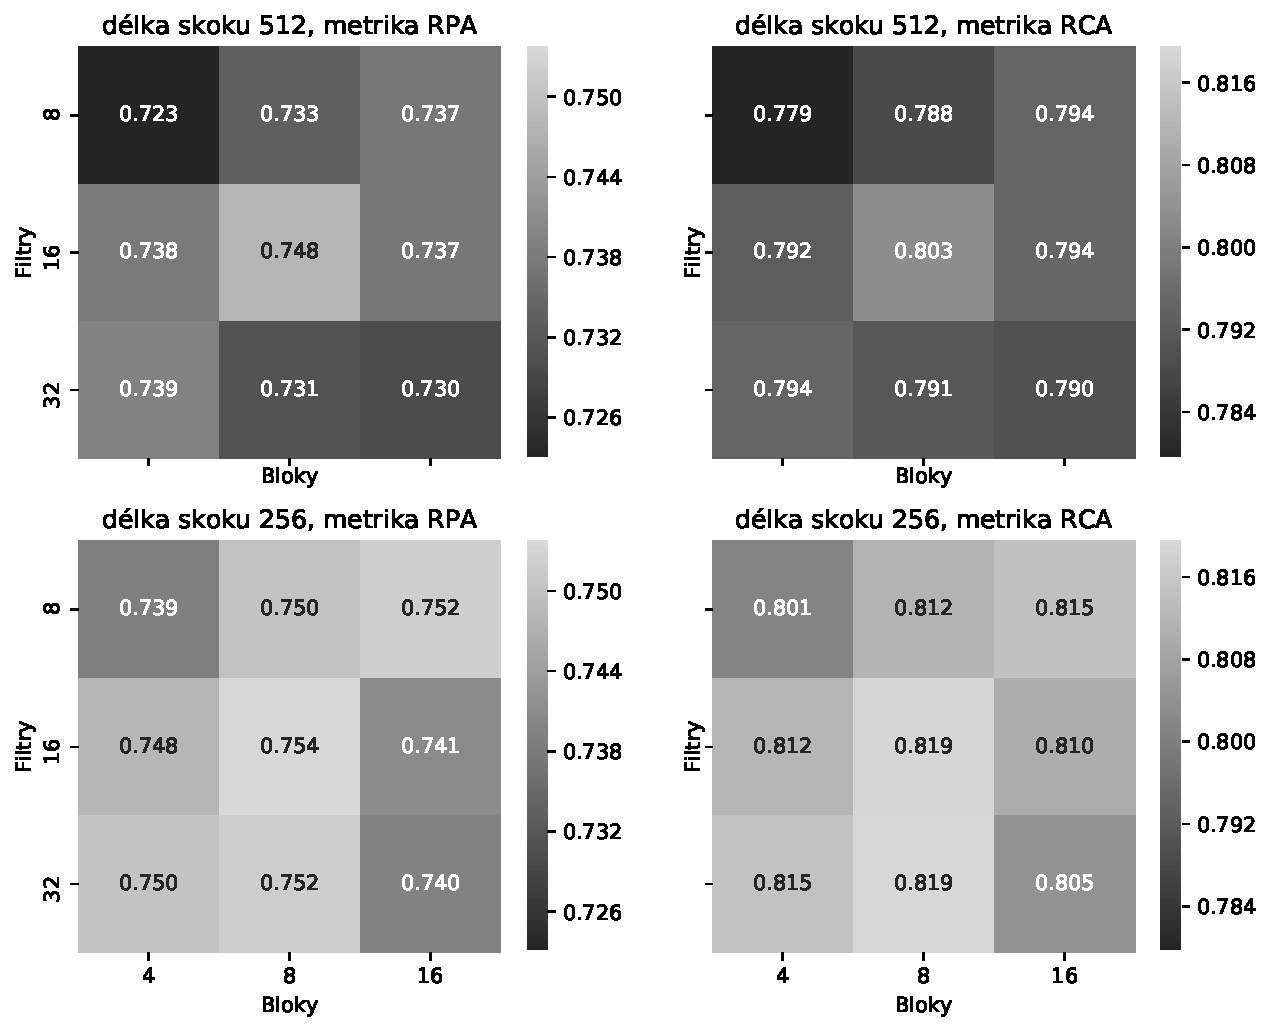
\includegraphics[scale=0.55]{../img/figures/spectrogram_512_vs_256_grey}
\caption{Architektura HCNN, Vliv velikosti skoku pro výpočet vstupního spektrogramu}\label{obr:spectrogram_512_vs_256}
\end{figure}

Výsledek prezentovaný na obrázku \ref{obr:spectrogram_512_vs_256} je potenciálně využitelný i pro metodu \cite{Bittner2017}. Je možné, že pokud se původní architektura přetrénuje na datech s menším \texttt{hop\_size}, výsledky sítí se také zvýší, jako v našem případě.

\subsection{Vícekanálový vstup CQT}\label{exp:hcnn_multichannel}

Při výpočtu CQT spektrogramu je možné nastavit parametr \texttt{filter\_scale}, což je koeficient ovlivňující velikost okna transformace. S menší velikostí okna se pojí lepší časové rozlišení, s větší naopak lepší frekvenční. Otestujeme proto sítě, které mají na vstupu k dispozici více variant CQT spektrogramu. Další možností úpravy vstupního spektrogramu je druh práhování nastavitelný parametrem \texttt{top\_db} ve funkci \texttt{librosa.core.amplitude\_to\_db}, prozkoumáme i tato nastavení. Vstupní vícekanálový spektrogram se proto bude skládat ze tří spektrogramů s dvojicemi parametrů \texttt{filter\_scale}, \texttt{top\_db}: (0.5, 60), (1, 80), (2, 100).

\begin{figure}[h]\centering
    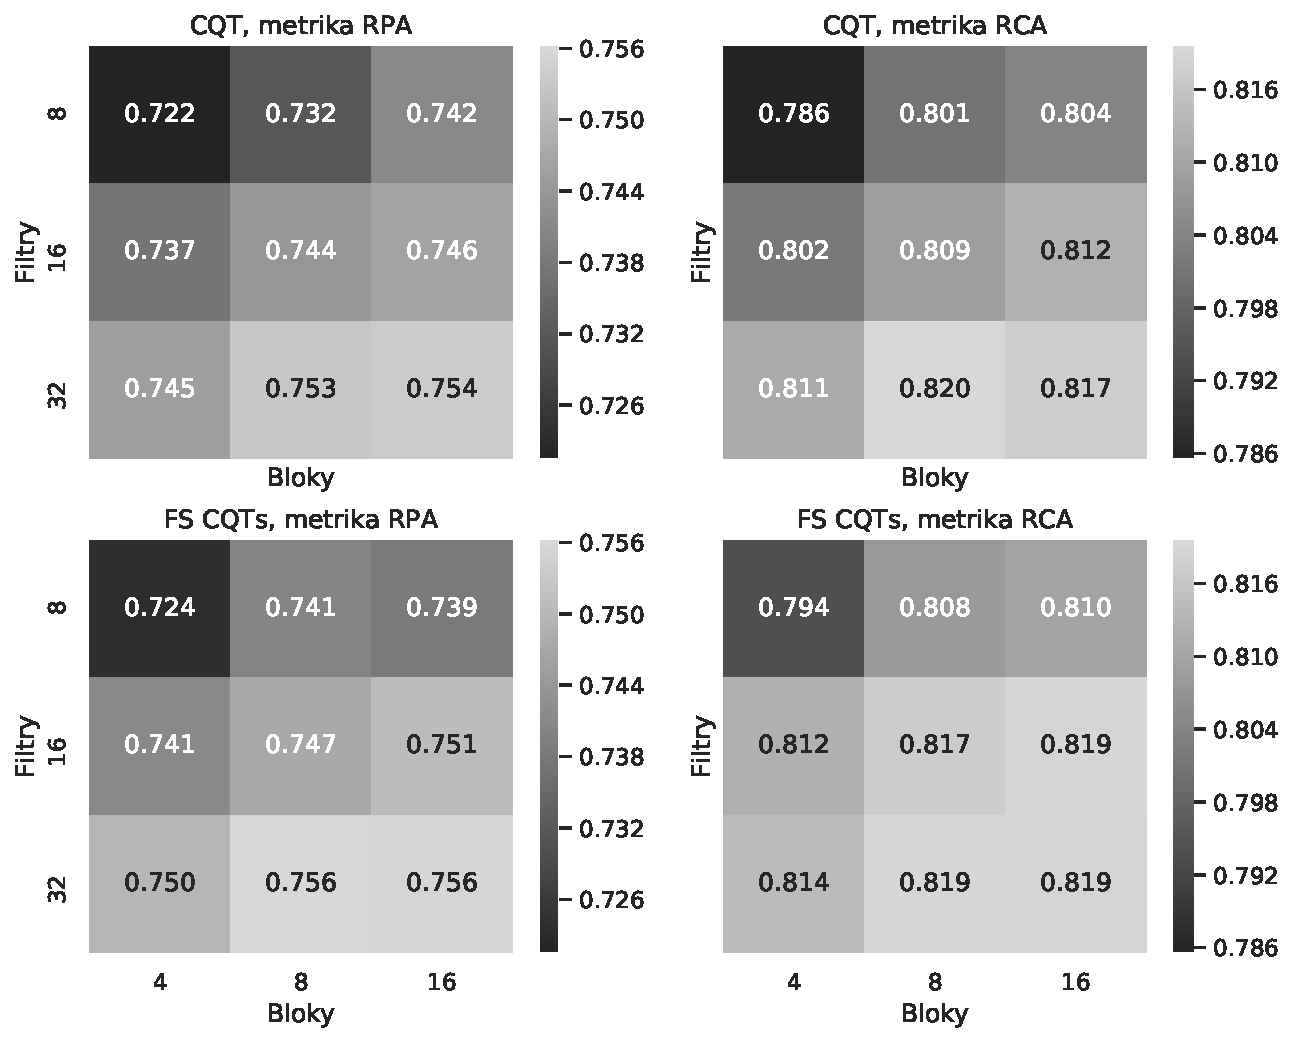
\includegraphics[scale=0.55]{../img/figures/spectrogram_fscqt_grey}
\caption{Architektura HCNN, Vliv vstupního vícekanálového CQT}\label{obr:spectrogram_fscqt}
\end{figure}

Výsledné zlepšení se pohybuje v desetinách procentního bodu u většiny testovaných konfigurací. Na druhou stranu vstupní reprezentace je nezávislá na architektuře zbytku modelu, tudíž je zde naděje, že toto zlepšení bude nezávislé na zvolené architektuře. Použití tohoto vstupu by tedy mohlo vylepšit i výsledky nejlepších objevených architektur.

% \subsection{Výška konvolucí}

% Otestujeme vliv velikosti konvoluce na frekvenční ose změnou velikosti kernelu z 1x3 na 1x4 a na 1x5 (viz obrázek \ref{obr:hcnn_layer}). Protože na jeden půltón připadá v používané vstupní reprezentaci 5 frekvenčních složek, volba větší konvoluce se zdá logická. Na druhou stranu dvě následující vrstvy 1x3 mají receptivní pole ekvivalentní velikosti při menším počtu.

% \textcolor{red}{trénuje se}

\subsection{Kontext}

Doposud jsme trénovali sítě, které pro výpočet salience uvažovaly pouze jedno okno vstupního CQT. Tyto sítě pro odhad výšky měly k dispozici pouze okno šířky $\approx 5.8\,\rm ms$. Následující sadou experimentů se pokusíme prozkoumat možnosti zvětšení tohoto kontextu. Všechny úpravy spočívají ve změnách konvolučních vrstev v blocích architektury (viz obrázek \ref{obr:hcnn_context_archs}), konkrétně nastavujeme velikost konvoluce z 1x3 na jiné hodnoty. Také prozkoumáváme možnost využití dilatovaných konvolucí, jejichž princip vysvětlujeme v sekci \nameref{sec:wavenet}, které umožňují snadno zvětšovat zpracovávaný kontext pomocí menšího počtu vrstev než s použitím obvyklých konvolucí.

\begin{figure}[h]\centering
    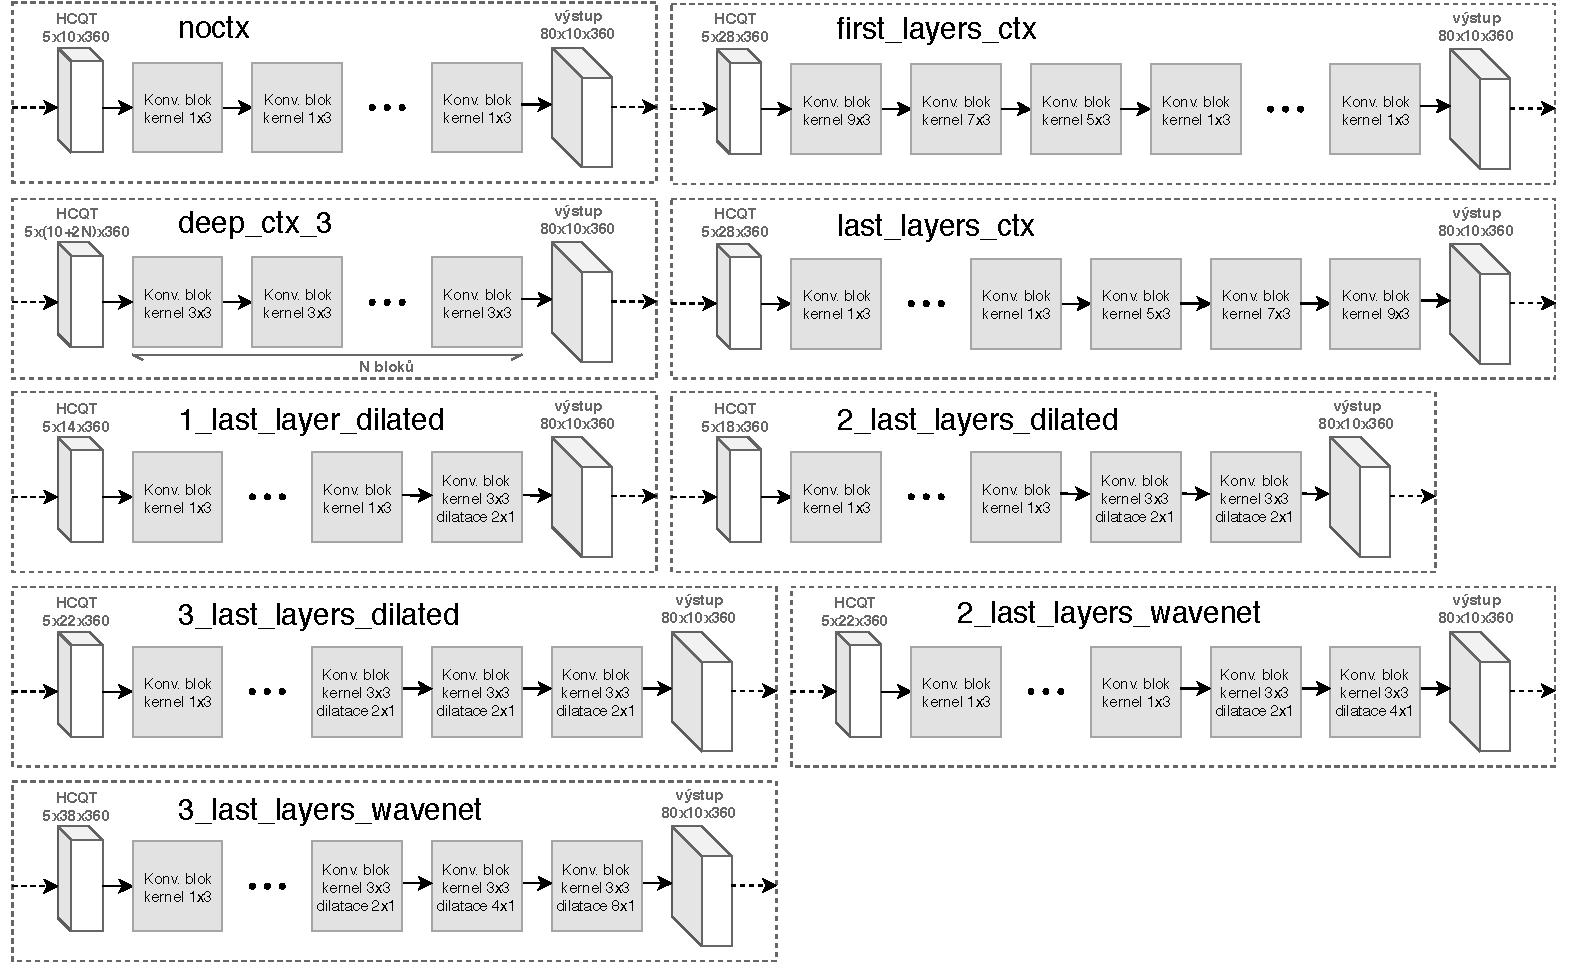
\includegraphics[width=\textwidth,height=\textheight,keepaspectratio]{../img/hcnn_context_archs_4_grey}
\caption{Úpravy architektury HCNN z obrázku \ref{obr:hcnn_arch} pro rozšíření uvažovaného kontextu.}\label{obr:hcnn_context_archs}
\end{figure}

Protože v předchozích experimentech dosahujeme vysoké úspěšnosti i bez použití kontextu navíc, ve většině testovaných architekturách zachováváme část této původní architektury a rozšíření receptivního pole zajišťují pouze poslední vrstvy. Testujeme tedy řadu různých změn architektur, pro každou variantu budeme trénovat verzi s celkově čtyřmi konvolučními bloky a s celkově osmi. Také každou variantu přetrénujeme ve verzi s 8 a s 16 konvolučními filtry v každém bloku. Celkově tedy budeme trénovat 4 varianty od každé architektury. Všechny sítě aplikují harmonickou transformaci $\pm 12$ v každém konvolučním bloku, vstupní reprezentací je HCQT s \texttt{hop\_size}=256. Testované architektury mají následující struktury:
\begin{itemize}
    \item  noctx: síť bez kontextu navíc, celkový kontext pro výpočet jednoho odhadu výšky je $5.8\,\rm ms$.
    \item  deep\_ctx\_3: síť s konvolucemi velikosti 3x3. Celkový kontext $2N \cdot 5.8\,\rm ms$ na jeden odhad je tedy dán hloubkou sítě $N$. Konkrétně tedy kontext vychází $46.4\,\rm ms$ pro verzi se čtyřmi konvolučními bloky a $92.8\,\rm ms$ pro verzi s osmi.
    \item  first\_layers\_ctx: síť s konvolucemi velikosti 9x3, 7x3 a 5x3, které zpracovávají vstupní spektrogram, následované konvolucemi 1x3, které již kontext nerozšiřují. Celkový kontext vychází $(8+6+4) \cdot 5.8\,\rm ms = 104.4\,\rm ms$.
    \item  last\_layers\_ctx: síť zpracovávající vstup konvolucemi 1x3, následované řadou vrstev s konvolucemi 9x3, 7x3 a 5x3. Celkový kontext $104.4\,\rm ms$.
    \item  1\_last\_layer\_dilated: síť zpracovávající vstup konvolucemi 1x3, následované jednou konvoluční vrstvou 3x3 s dilatací 2 v dimenzi času. Celkový kontext $23.2\,\rm ms$.
    \item  2\_last\_layers\_dilated: síť zpracovávající vstup konvolucemi 1x3, následované dvěma konvolučními vrstvami 3x3 s dilatací 2 v dimenzi času. Celkový kontext $46.4\,\rm ms$.
    \item  3\_last\_layers\_dilated: síť zpracovávající vstup konvolucemi 1x3, následované třemi konvolučními vrstvami 3x3 s dilatací 2 v dimenzi času. Celkový kontext $69.6\,\rm ms$.
    \item  2\_last\_layers\_wavenet: síť zpracovávající vstup konvolucemi 1x3, následované dvěma konvolučními vrstvami 3x3 s dilatacemi 2 a 4 v dimenzi času. Celkový kontext $69.6\,\rm ms$.
    \item  3\_last\_layers\_wavenet: síť zpracovávající vstup konvolucemi 1x3, následované třemi konvolučními vrstvami 3x3 s dilatacemi 2, 4 a 8 v dimenzi času. Celkový kontext $162.4\,\rm ms$.
\end{itemize}
\begin{figure}[h]\centering
    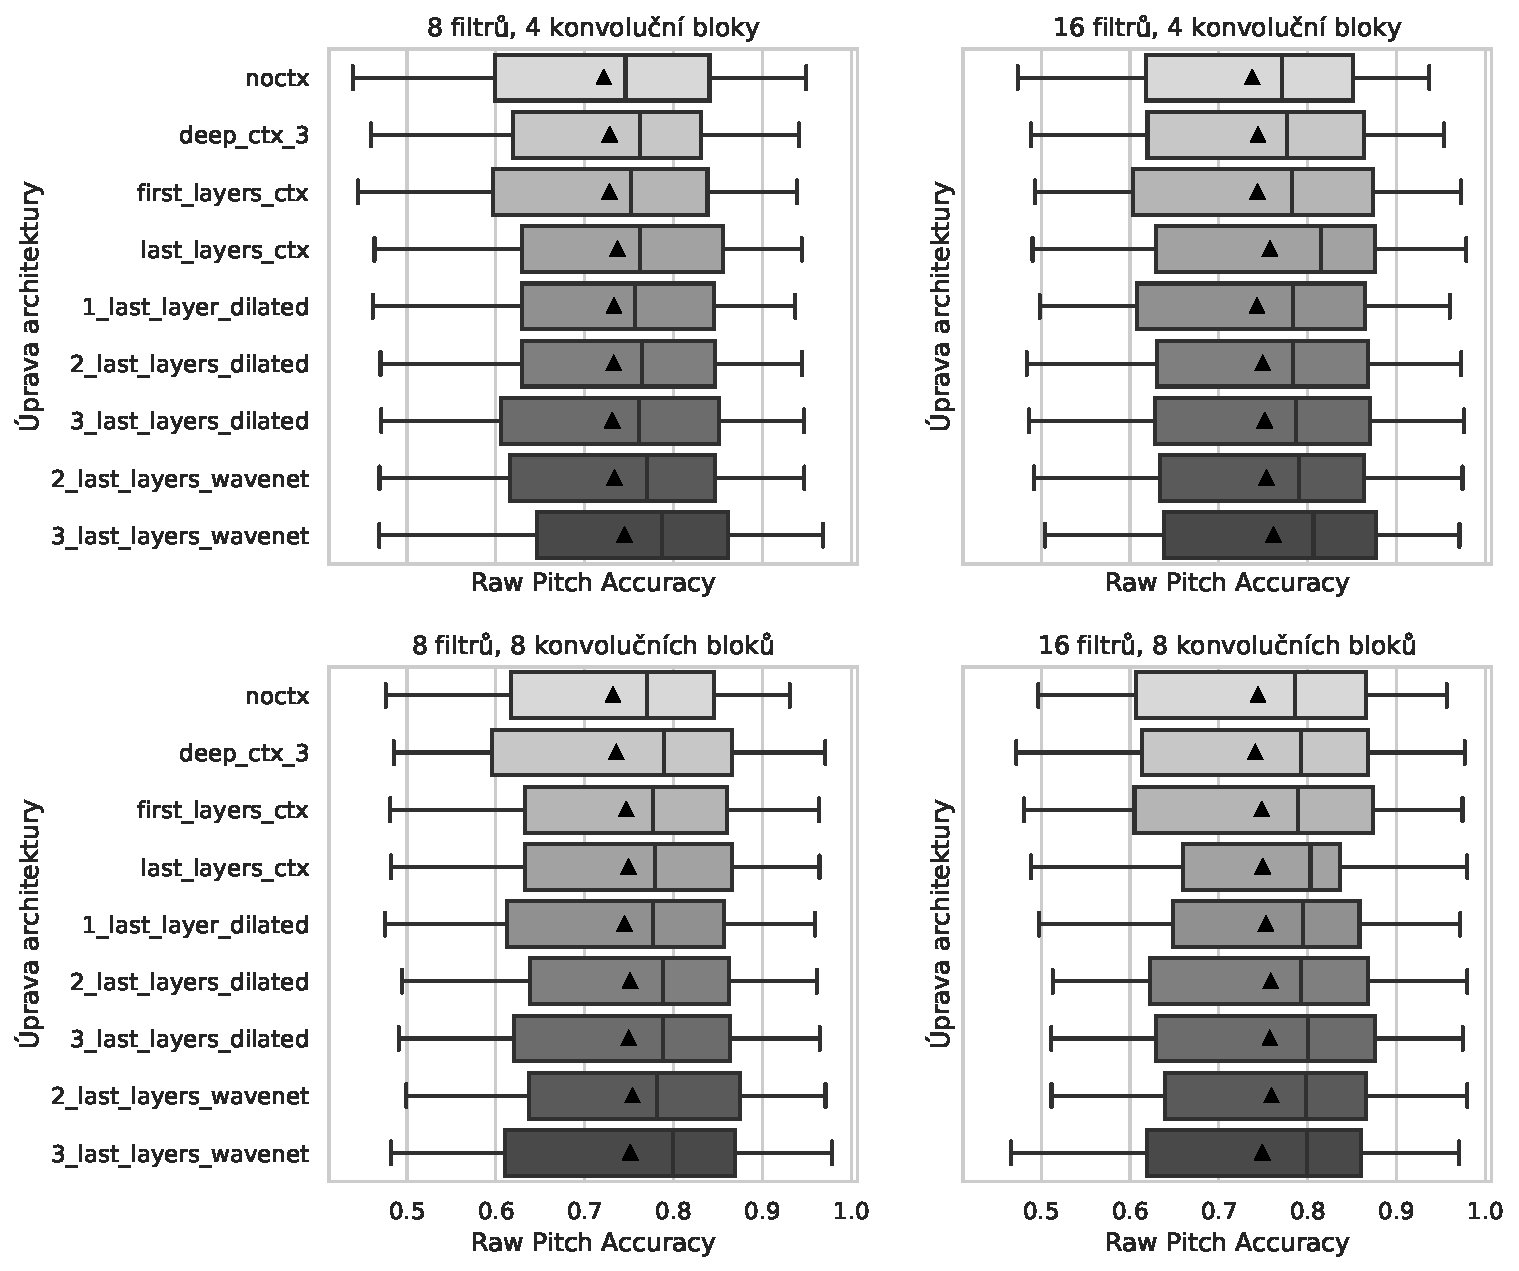
\includegraphics[width=\textwidth,height=\textheight,keepaspectratio]{../img/figures/spectrogram_ctx_archs_grey}
\caption{Architektura HCNN, Vliv úpravy architektury ovlivňující receptivní pole modelu.}\label{obr:spectrogram_ctx_archs}
\end{figure}

Poznamenáme také, že šířka vstupních spektrogramů v ose času je pro každý experiment rozšířena tak, aby konvoluční bloky měly k dispozici všechny potřebné informace pro výpočet hodnot na výstupním oknu. Například pokud tedy síť pro jeden bod anotace využívá také tři předcházející a tři nadcházející okna spektrogramu, rozšíříme vstupní spektrogram z obou stran o tři okna.


Výsledky uvádíme na obrázku \ref{obr:spectrogram_ctx_archs}, kvůli většímu rozměru tabulku s výsledky přesouváme do přílohy \ref{appendix:hcnn_ctx}. Prvním důležitým pozorováním je, že přidaný kontext oproti kontrolní síti bez kontextu výsledky sítí zlepšuje téměř ve všech případech. Sítě tedy jsou schopné přidaný kontext využít k lepším odhadům. Dále vidíme, že síť deep\_ctx\_3 si vede nejhůře ze všech testovaných, tato síť na rozdíl od ostatních neobsahuje žádné konvoluce 1x3, můžeme se tedy domnívat, že konvoluce 3x3 na datech v této architektuře nefungují natolik dobře, jako jejich užší varianty. Je však také možné, že informace o kontextu je pro síť obtížné využít, pokud tato informace má projít dlouhou kaskádou úzkých konvolucí, na které se architektura deep\_ctx\_3 zakládá.

Nejlepší výsledek podává mělká architektura se čtyřmi bloky, jde o konfiguraci s 16 filtry, 4 konvolučními bloky a architekturou 3\_last\_layers\_wavenet, tato architektura tedy obsahuje pouze jednu konvoluční vrstvu šířky 1x3 a pak následují dilatované konvoluce 3x3.

\subsection{Augmentace vstupních spektrogramů}

\begin{figure}[h]\centering
    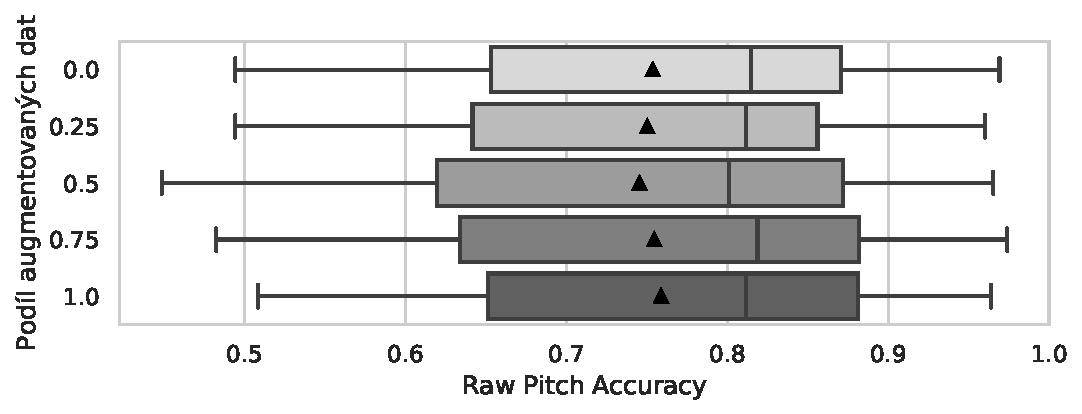
\includegraphics[scale=0.6]{../img/figures/spectrogram_specaugment_grey}
\caption{Architektura HCNN, vliv použití SpecAugment na vstupní spektrogramy.}\label{obr:hcnn_specaugment}
\end{figure}

\begin{table}[h]
\centering
    \begin{tabular}{lrr}
    \toprule
    Podíl augmentovaných dat &   RPA &   RCA \\
    \midrule
                        0.0 & 0.754 & 0.818 \\
                        0.25 & 0.750 & 0.824 \\
                        0.5 & 0.745 & 0.820 \\
                        0.75 & 0.755 & 0.828 \\
                        1.0 & 0.759 & 0.824 \\
    \bottomrule
    \end{tabular}
\caption{Architektura HCNN, vliv použití SpecAugment na vstupní spektrogramy.}\label{tab:hcnn_specaugment}
\end{table}

Jak shrnujeme v kapitole \nameref{cha:souvisejici}, metody, které používají hlubokého učení k extrakci melodie, také často prozkoumávají možnosti augmentace vstupních dat, aby snížily míru přeučení svých modelů. Prozkoumáme proto zběžně novou techniku augmentace nazvanou SpecAugment, která byla představena v článku \cite{Park2019} a je určena pro úpravu vstupních časově-frekvenčních reprezentací. Augmentace je v principu velmi jednoduchá, spočívá ve vynechání náhodně zvolených frekvenčních pásem a časových úseků na vstupu sítě. Díky tomu se trénovaný model stává odolnější vůči neúplným a zkresleným příkladům. Na síť je také následně možné nahlížet i perspektivou generativních modelů, ve které se model snaží v místě chybějících informací predikovat příklad výstupu z distribuce podmíněné vstupním zvukovým okolím. Jinou motivací také může být paralela s lidským vnímáním, lidský sluch je totiž vůči vynechání frekvenčních pásem také odolný, zvuk po aplikaci pásmového filtru sice zní pozměněně, nicméně kvality jako je výška tónu si zachovává. Vzhledem ke stáří tohoto článku představujeme první pokus o aplikaci této augmentace na melodická data. Augmentaci testujeme na nejlepší síti z minulé sekce, tedy na architektuře 3\_last\_layers\_wavenet s 16 filtry a 4 konvolučními bloky. Navíc síti předkládáme vícekanálový vstup popsaný v sekci \nameref{exp:hcnn_multichannel}.

Z článku SpecAugment implementujeme vynechávání frekvenčních pásem a časových úseků. Náhodnou část vstupních spektrogramů transformujeme ve frekvenční doméně překrytím dvou frekvenčních pásem šířky až 5.4 půltónu, v časové doméně pak vynecháváme jeden úsek délky až $29\,\rm ms$.


Výsledky nalezneme v tabulce \ref{tab:hcnn_specaugment} a na obrázku \ref{obr:hcnn_specaugment}. Pro tuto síť se rozdíl mezi výsledky sítě bez augmentace vstupních dat a se vstupem pouze augmentovaných dat pohybuje kolem půl procentního bodu. Vzhledem k výsledkům prezentovaným v článku \cite{Park2019} se však domníváme, že augmentace má vyšší potenciál, zejména pak pro větší sítě s delším kontextem, které mají větší tendence k přeučení.

% section{Detekce melodie}

% \begin{figure}[h]\centering
%     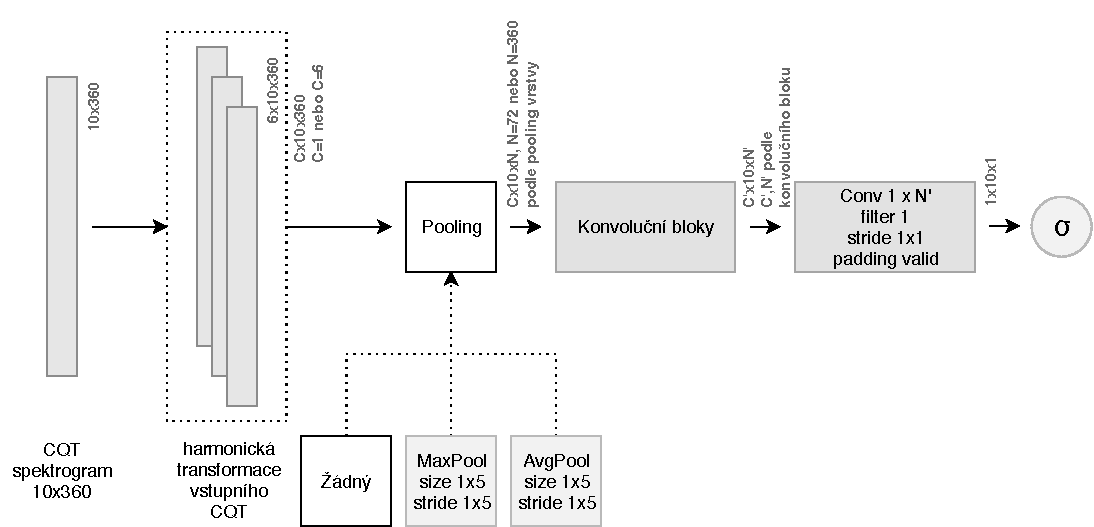
\includegraphics[width=\textwidth,height=\textheight,keepaspectratio]{../img/voicing_struktura_grey}
% \caption{Diagram společné struktury modelů pro detekci melodie.}\label{obr:voicing_struktura}
% \end{figure}

% Podobně jako v práci \cite{Rigaud2016} jsme otestovali možnosti oddělení modulu pro odhad výšky melodie a pro její detekci. V této sekci proto nejprve provedeme sadu experimentů, ve kterých návrhy na modul pro detekci trénujeme samostatně a poté otestujeme jeho přesnost také v kombinaci s modulem pro 16 filtrů, 8 konv. blokůšky.

% Při hledání nejlepší architektury pro detekci jsme postupovali iterativním prohlubování návrhů sítí. Společná struktura všech experimentů je znázorněna na diagramu \ref{obr:voicing_struktura}. Vstupem modelů je CQT spektrogram, podobně jako pro modely HCNN. Ten v některých experimentech transformujeme pomocí harmonického posunu (viz diagram \ref{obr:hcnn_harmonic_stacking}). Dále tento spektrogram potenciálně zmenšíme pomocí jedné pooling vrstvy tak, aby na jeden půltón připadala jedna složka výstupu, u většiny experimetů však tuto transformaci vynecháváme. Tento upravený vstup pak zpracováváme jedním z konvolučních bloků znázorněných na obrázku \ref{obr:voicing_moduly}. Výstup bloku pomocí konvoluce a následné sigmoidy zredukujeme na výstupní hodnoty označující přítomnost melodie v každém ze vstupních oken. 

% V diagramu konvolučních bloků \ref{obr:voicing_moduly} obsahují bloky \texttt{dilated\_block}, \texttt{octave\_block} a \texttt{note\_block} podsoučást \texttt{reg. blok}, tedy regularizační blok. Ten se skládá z kombinace dropout vrstvy a batch normalizace, nejvýhodnější kombinaci budeme ověřovat experimentálně. Dále také na obrázku používáme proměnné $\mathbf{ T_{CTX}}$ pro parametrizaci šířky konvolucí a $\mathbf{K}$ multiplikační koeficient kapacity. Nastavení těchto proměnných budeme také porovnávat v následujících podsekcích. Dále se v diagramech používá proměnná N, která je vázaná na šířku vstupu daného bloku. 

% Úlohu detekce formulujeme jako binární klasifikaci pro každé uvažované vstupní okno signálu. Síť je trénována pomocí vzájemné korelace mezi výstupem a cílovou množinou binárních veličin, které indikují přítomnost melodie.


% \begin{figure}[h]\centering
%     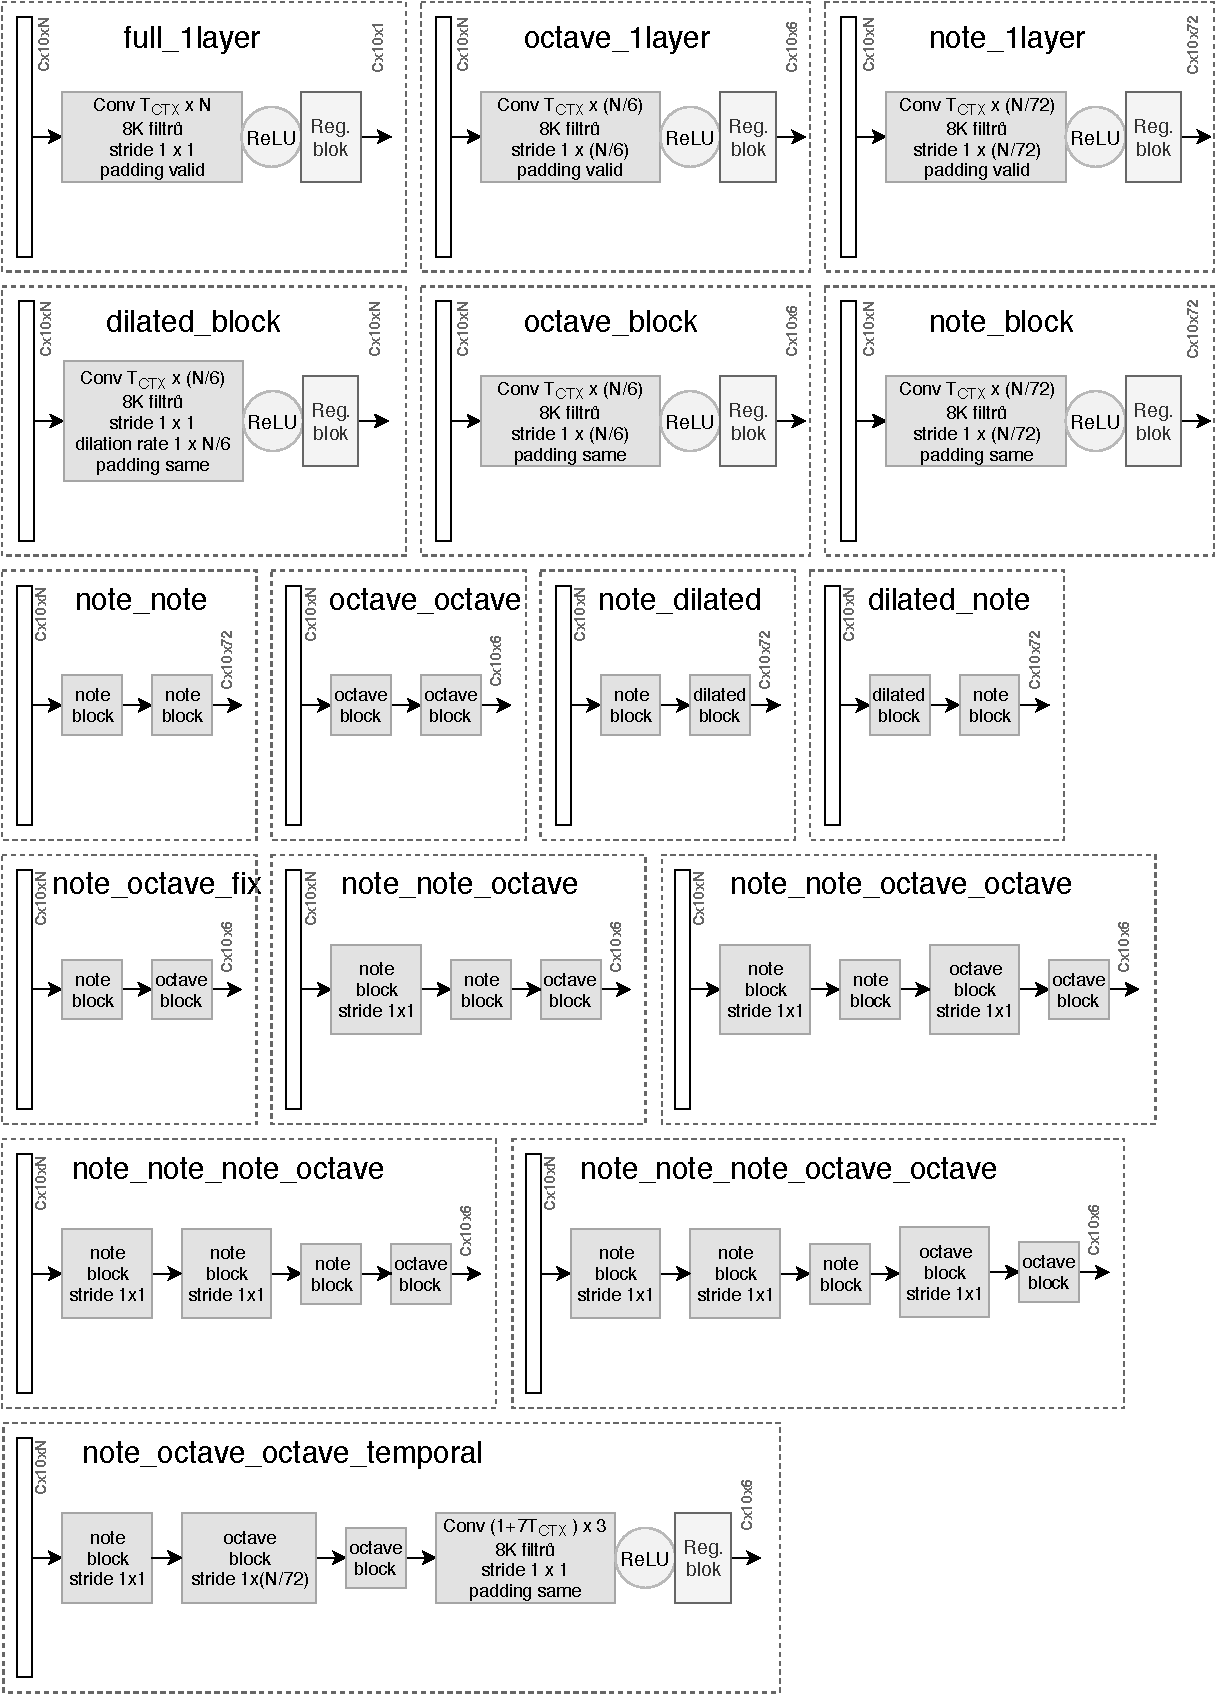
\includegraphics[width=\textwidth,height=\textheight,keepaspectratio]{../img/voicing_moduly_grey}
% \caption{Diagram testovaných druhů konvolučních bloků pro detekci melodie.}\label{obr:voicing_moduly}
% \end{figure}

% \subsection{Vliv počáteční pooling vrstvy}

% Motivací pro použití pooling vrstvy je zmenšení nejspíše zbytečně podrobné frekvenční dimenze vstupu. Protože výstup úlohy detekce melodie nemusí obsahovat přesnou informaci o výšce tónu, pouze binární informaci o její přítomnosti v daném časovém okamžiku, jemná frekvenční osa se zdá redundantní a ponechání plného rozlišení vede ke zbytečně větším modelům. Pomocí experimentů na sadě architektur se proto pokusíme ověřit vliv této redukce.

% \begin{table}[h!]
% \centering
%     \begin{tabular}{llrrr}
%     \toprule
%             Model & Pooling &    VR &   VFA &    VA \\
%     \midrule
%     full\_1layer &    None & 0.818 & 0.606 & 0.616 \\
%     full\_1layer &     avg & 0.820 & 0.600 & 0.616 \\
%     full\_1layer &     max & 0.830 & 0.589 & 0.628 \\
%     note\_1layer &    None & 0.722 & 0.451 & 0.636 \\
%     note\_1layer &     avg & 0.751 & 0.547 & 0.605 \\
%     note\_1layer &     max & 0.733 & 0.477 & 0.626 \\
%     note\_dilated &    None & 0.720 & 0.441 & 0.636 \\
%     note\_dilated &     avg & 0.680 & 0.473 & 0.595 \\
%     note\_dilated &     max & 0.668 & 0.413 & 0.617 \\
%         note\_note &    None & 0.701 & 0.401 & 0.648 \\
%         note\_note &     avg & 0.722 & 0.519 & 0.602 \\
%         note\_note &     max & 0.682 & 0.436 & 0.619 \\
%     octave\_1layer &    None & 0.789 & 0.523 & 0.638 \\
%     octave\_1layer &     avg & 0.793 & 0.527 & 0.634 \\
%     octave\_1layer &     max & 0.809 & 0.561 & 0.628 \\
%     octave\_octave &    None & 0.588 & 0.337 & 0.617 \\
%     octave\_octave &     avg & 0.709 & 0.454 & 0.624 \\
%     octave\_octave &     max & 0.740 & 0.473 & 0.632 \\
%     \bottomrule
%     \end{tabular}
% \caption{Detekce melodie, vliv počáteční pooling vrstvy.}\label{tab:voicing_pooling}
% \end{table}

% \begin{figure}[h]\centering
%     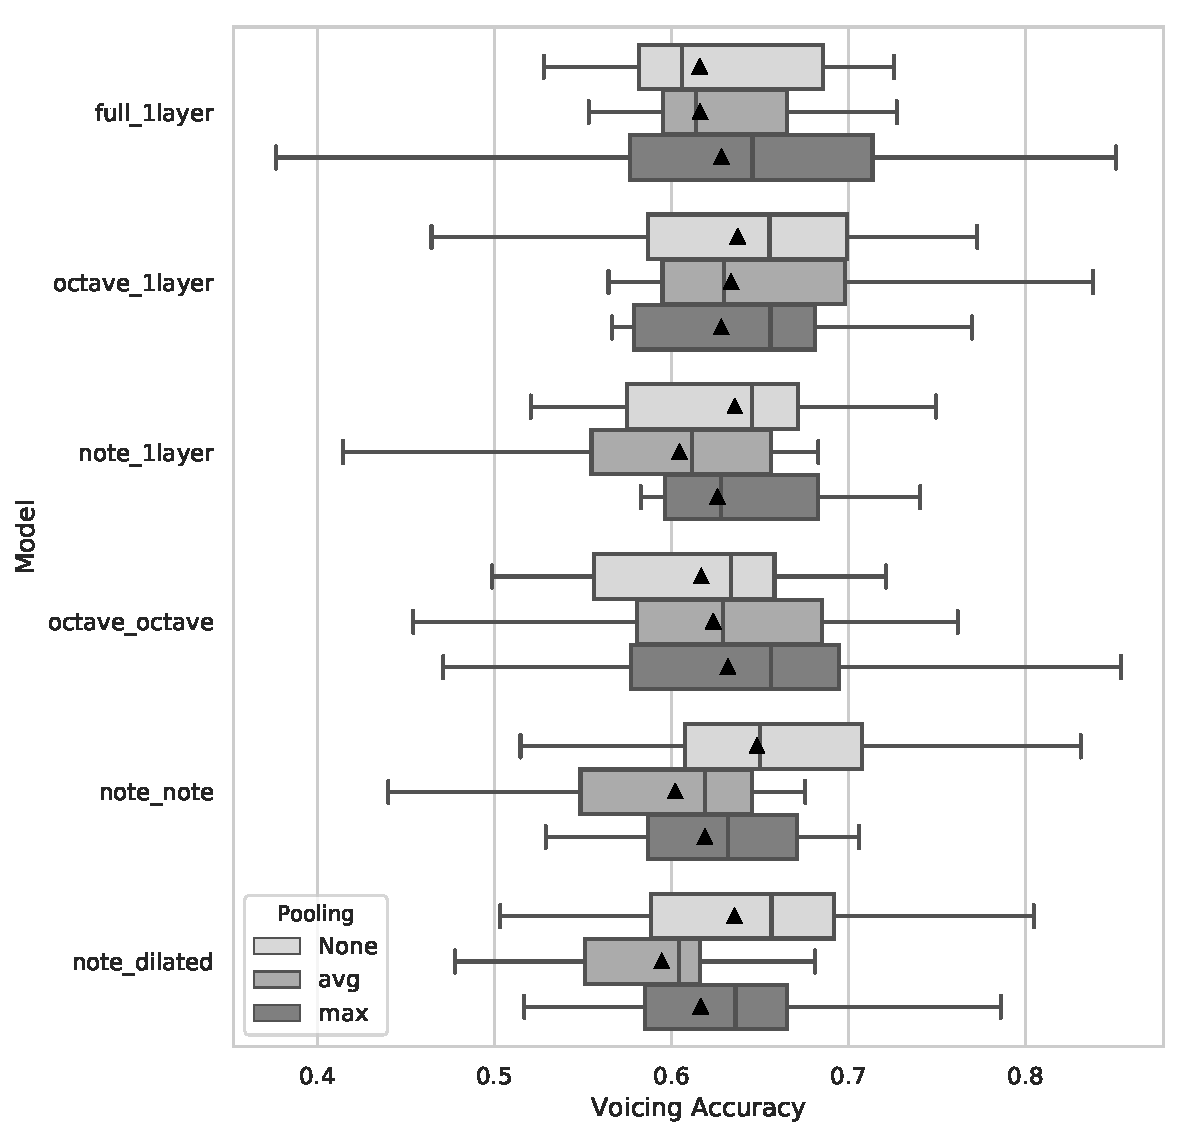
\includegraphics[scale=0.6]{../img/figures/voicing_pooling_grey}
% \caption{Detekce melodie, vliv počáteční pooling vrstvy.}\label{obr:voicing_pooling}
% \end{figure}

% Z tabulky \ref{tab:voicing_pooling} a obrázku \ref{obr:voicing_pooling} vidíme, že u většiny experimentů zpracování vstupu pooling vrstvou spíše zhoršilo, v dalších experimentech proto zpracování pooling vrstvou nepoužíváme.

% \subsection{Vliv použití dropout jako regularizace}

% Sadou experimentů prozkoumáme účinnost regularizace pomocí dropout vrstvy po každé konvoluční vrstvě v modelu. Parametr pravděpodobnosti vynechání složky jsme nastavili na $0.3$. 

% \begin{table}[h!]
% \centering
%     \begin{tabular}{llrrr}
%     \toprule
%             Model & Dropout &    VR &   VFA &    VA \\
%     \midrule
%     full\_1layer &     0.0 & 0.782 & 0.565 & 0.618 \\
%     full\_1layer &     0.3 & 0.825 & 0.632 & 0.610 \\
%     octave\_1layer &     0.0 & 0.610 & 0.357 & 0.625 \\
%     octave\_1layer &     0.3 & 0.832 & 0.586 & 0.629 \\
%     note\_1layer &     0.0 & 0.691 & 0.418 & 0.634 \\
%     note\_1layer &     0.3 & 0.791 & 0.519 & 0.642 \\
%     octave\_octave &     0.0 & 0.588 & 0.337 & 0.617 \\
%     octave\_octave &     0.3 & 0.824 & 0.564 & 0.636 \\
%         note\_note &     0.0 & 0.743 & 0.438 & 0.648 \\
%         note\_note &     0.3 & 0.758 & 0.424 & 0.666 \\
%     note\_dilated &     0.0 & 0.720 & 0.441 & 0.636 \\
%     note\_dilated &     0.3 & 0.686 & 0.362 & 0.656 \\
%     \bottomrule
%     \end{tabular}
% \caption{Detekce melodie, vliv dropout vrstvy.}\label{tab:voicing_dropout}
% \end{table}

% \begin{figure}[h]\centering
%     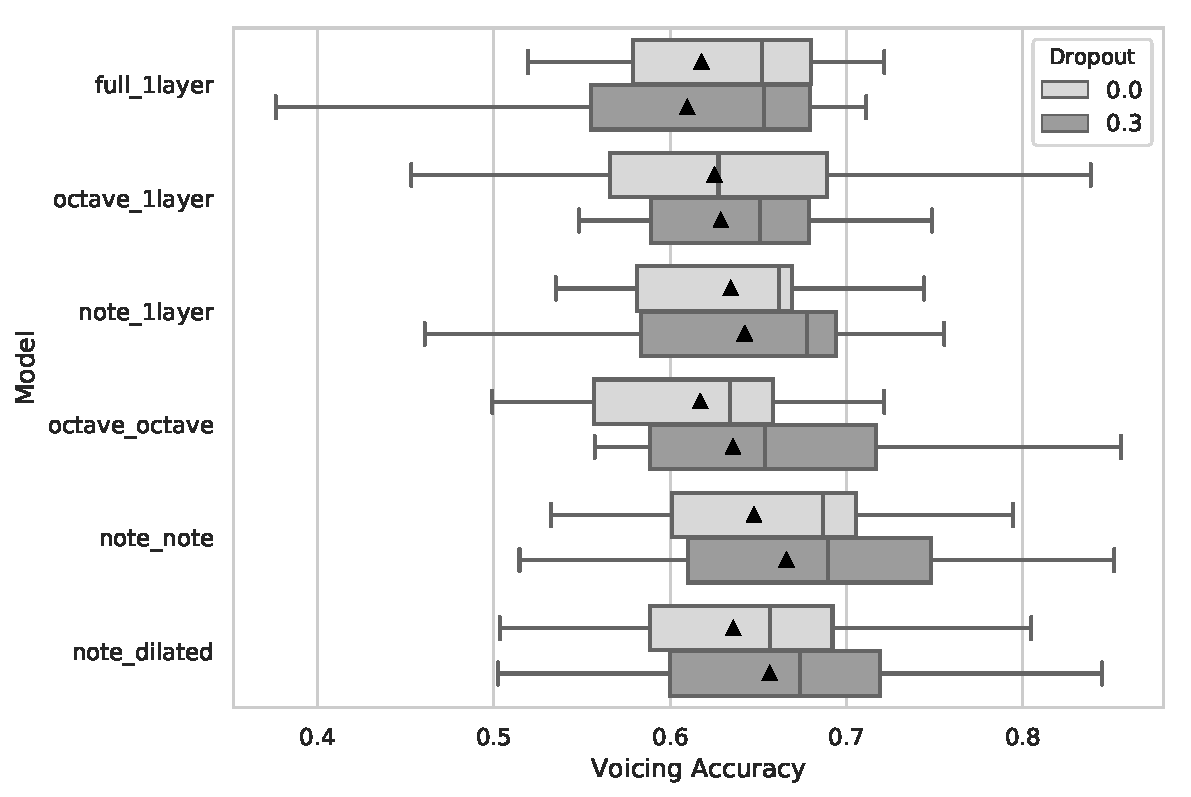
\includegraphics[scale=0.6]{../img/figures/voicing_dropout_grey}
% \caption{Detekce melodie, vliv dropout vrstvy.}\label{obr:voicing_dropout}
% \end{figure}

% Výsledky experimentů můžeme porovnat na obrázku \ref{obr:voicing_dropout} a v tabulce \ref{tab:voicing_dropout}, dropout vrstva výrazně pomáhá zvýšit přesnost modelu, zejména pak u architektur se dvěma vrstvami. V následujících experimentech dropout proto používáme.

% \subsection{Vliv použití batch normalizace jako regularizace}

% Sadou experimentů prozkoumáme účinnost regularizace pomocí batch normalizace po každé konvoluční vrstvě v modelu. 

% \begin{table}[h!]
% \centering
%     \begin{tabular}{llrrr}
%     \toprule
%             Model & Batch normalizace &    VR &   VFA &    VA \\
%     \midrule
%     full\_1layer &        Ne & 0.849 & 0.678 & 0.598 \\
%     full\_1layer &        Ano & 0.825 & 0.632 & 0.610 \\
%     note\_1layer &        Ne & 0.767 & 0.485 & 0.644 \\
%     note\_1layer &        Ano & 0.791 & 0.519 & 0.642 \\
%     note\_dilated &        Ne & 0.720 & 0.426 & 0.646 \\
%     note\_dilated &        Ano & 0.686 & 0.362 & 0.656 \\
%         note\_note &        Ne & 0.761 & 0.439 & 0.659 \\
%         note\_note &        Ano & 0.758 & 0.424 & 0.666 \\
%     octave\_1layer &        Ne & 0.841 & 0.557 & 0.647 \\
%     octave\_1layer &        Ano & 0.832 & 0.586 & 0.629 \\
%     octave\_octave &        Ne & 0.845 & 0.607 & 0.631 \\
%     octave\_octave &        Ano & 0.824 & 0.564 & 0.636 \\
%     \bottomrule
%     \end{tabular}

% \caption{Detekce melodie, vliv batch normalizace.}\label{tab:voicing_batchnorm}
% \end{table}

% \begin{figure}[h]\centering
%     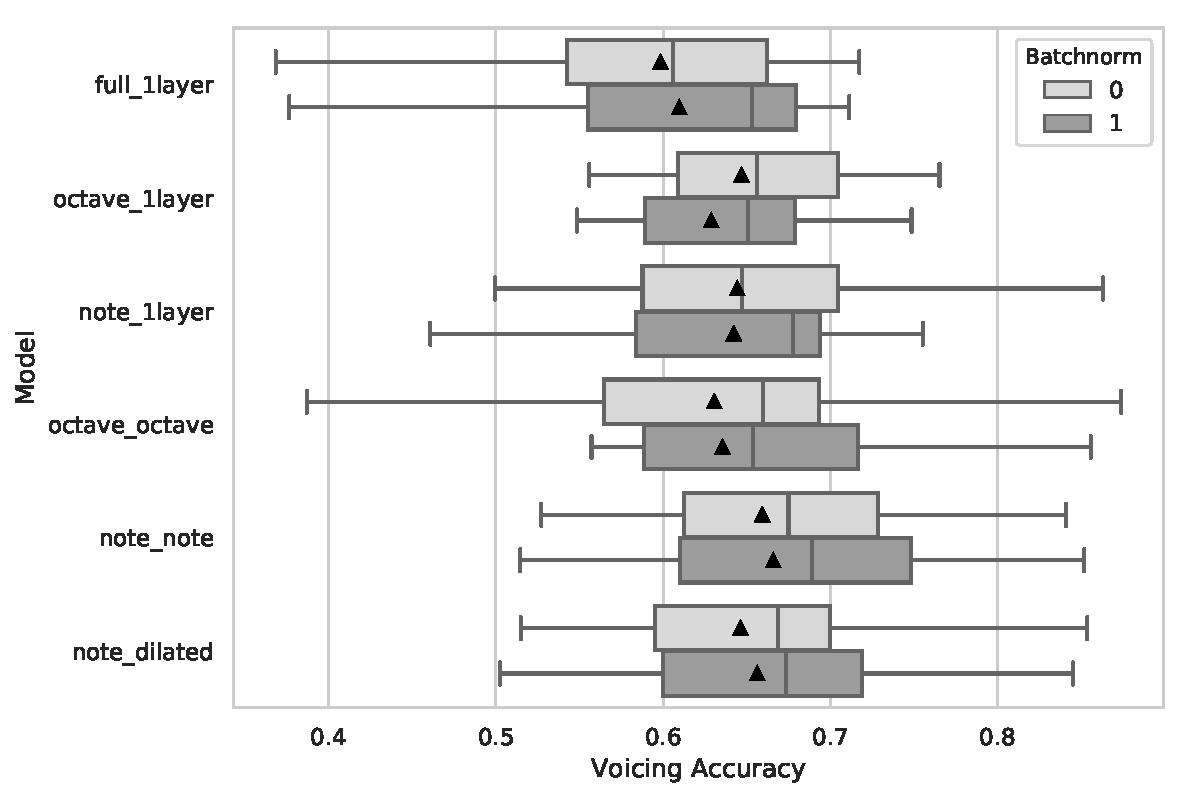
\includegraphics[scale=0.6]{../img/figures/voicing_batchnorm_grey}
% \caption{Detekce melodie, vliv batch normalizace.}\label{obr:voicing_batchnorm}
% \end{figure}

% Z výsledků na obrázku \ref{obr:voicing_batchnorm} a v tabulce \ref{tab:voicing_batchnorm} vyplývá, že batch normalizace přesnost sítí mírně zlepšuje, proto ji v následujících experimentech používáme společně s dropout regularizací.

% \subsection{Vliv kapacity sítě}

% Konstrukcí a natrénováním sítí s různou kapacitou nastavenou pomocí parametru $\mathbf{K}$ na diagramu \ref{obr:voicing_moduly} ověříme, jaký počet konvolučních filtrů je pro úlohu a danou architekturu vhodný. 

% \begin{table}[h!]
% \centering
%     \begin{tabular}{lrrrr}
%     \toprule
%             Model & Mult. Koef. Kapacity &    VR &   VFA &    VA \\
%     \midrule
%     full\_1layer &                    8 & 0.825 & 0.632 & 0.610 \\
%     full\_1layer &                   16 & 0.923 & 0.765 & 0.601 \\
%     full\_1layer &                   32 & 0.858 & 0.690 & 0.600 \\
%     note\_1layer &                    8 & 0.791 & 0.519 & 0.642 \\
%     note\_1layer &                   16 & 0.845 & 0.583 & 0.641 \\
%     note\_1layer &                   32 & 0.829 & 0.565 & 0.641 \\
%     note\_dilated &                    8 & 0.686 & 0.362 & 0.656 \\
%     note\_dilated &                   16 & 0.766 & 0.474 & 0.649 \\
%     note\_dilated &                   32 & 0.694 & 0.395 & 0.646 \\
%         note\_note &                    8 & 0.758 & 0.424 & 0.666 \\
%         note\_note &                   16 & 0.711 & 0.368 & 0.662 \\
%         note\_note &                   32 & 0.676 & 0.338 & 0.659 \\
%     octave\_1layer &                    8 & 0.832 & 0.586 & 0.629 \\
%     octave\_1layer &                   16 & 0.842 & 0.588 & 0.636 \\
%     octave\_1layer &                   32 & 0.859 & 0.612 & 0.634 \\
%     octave\_octave &                    8 & 0.824 & 0.564 & 0.636 \\
%     octave\_octave &                   16 & 0.799 & 0.487 & 0.659 \\
%     octave\_octave &                   32 & 0.648 & 0.343 & 0.640 \\
%     \bottomrule
%     \end{tabular}

% \caption{Detekce melodie, vliv batch normalizace.}\label{tab:voicing_capacity}
% \end{table}

% \subsection{Vliv kontextu}

% \begin{figure}[h]\centering
%     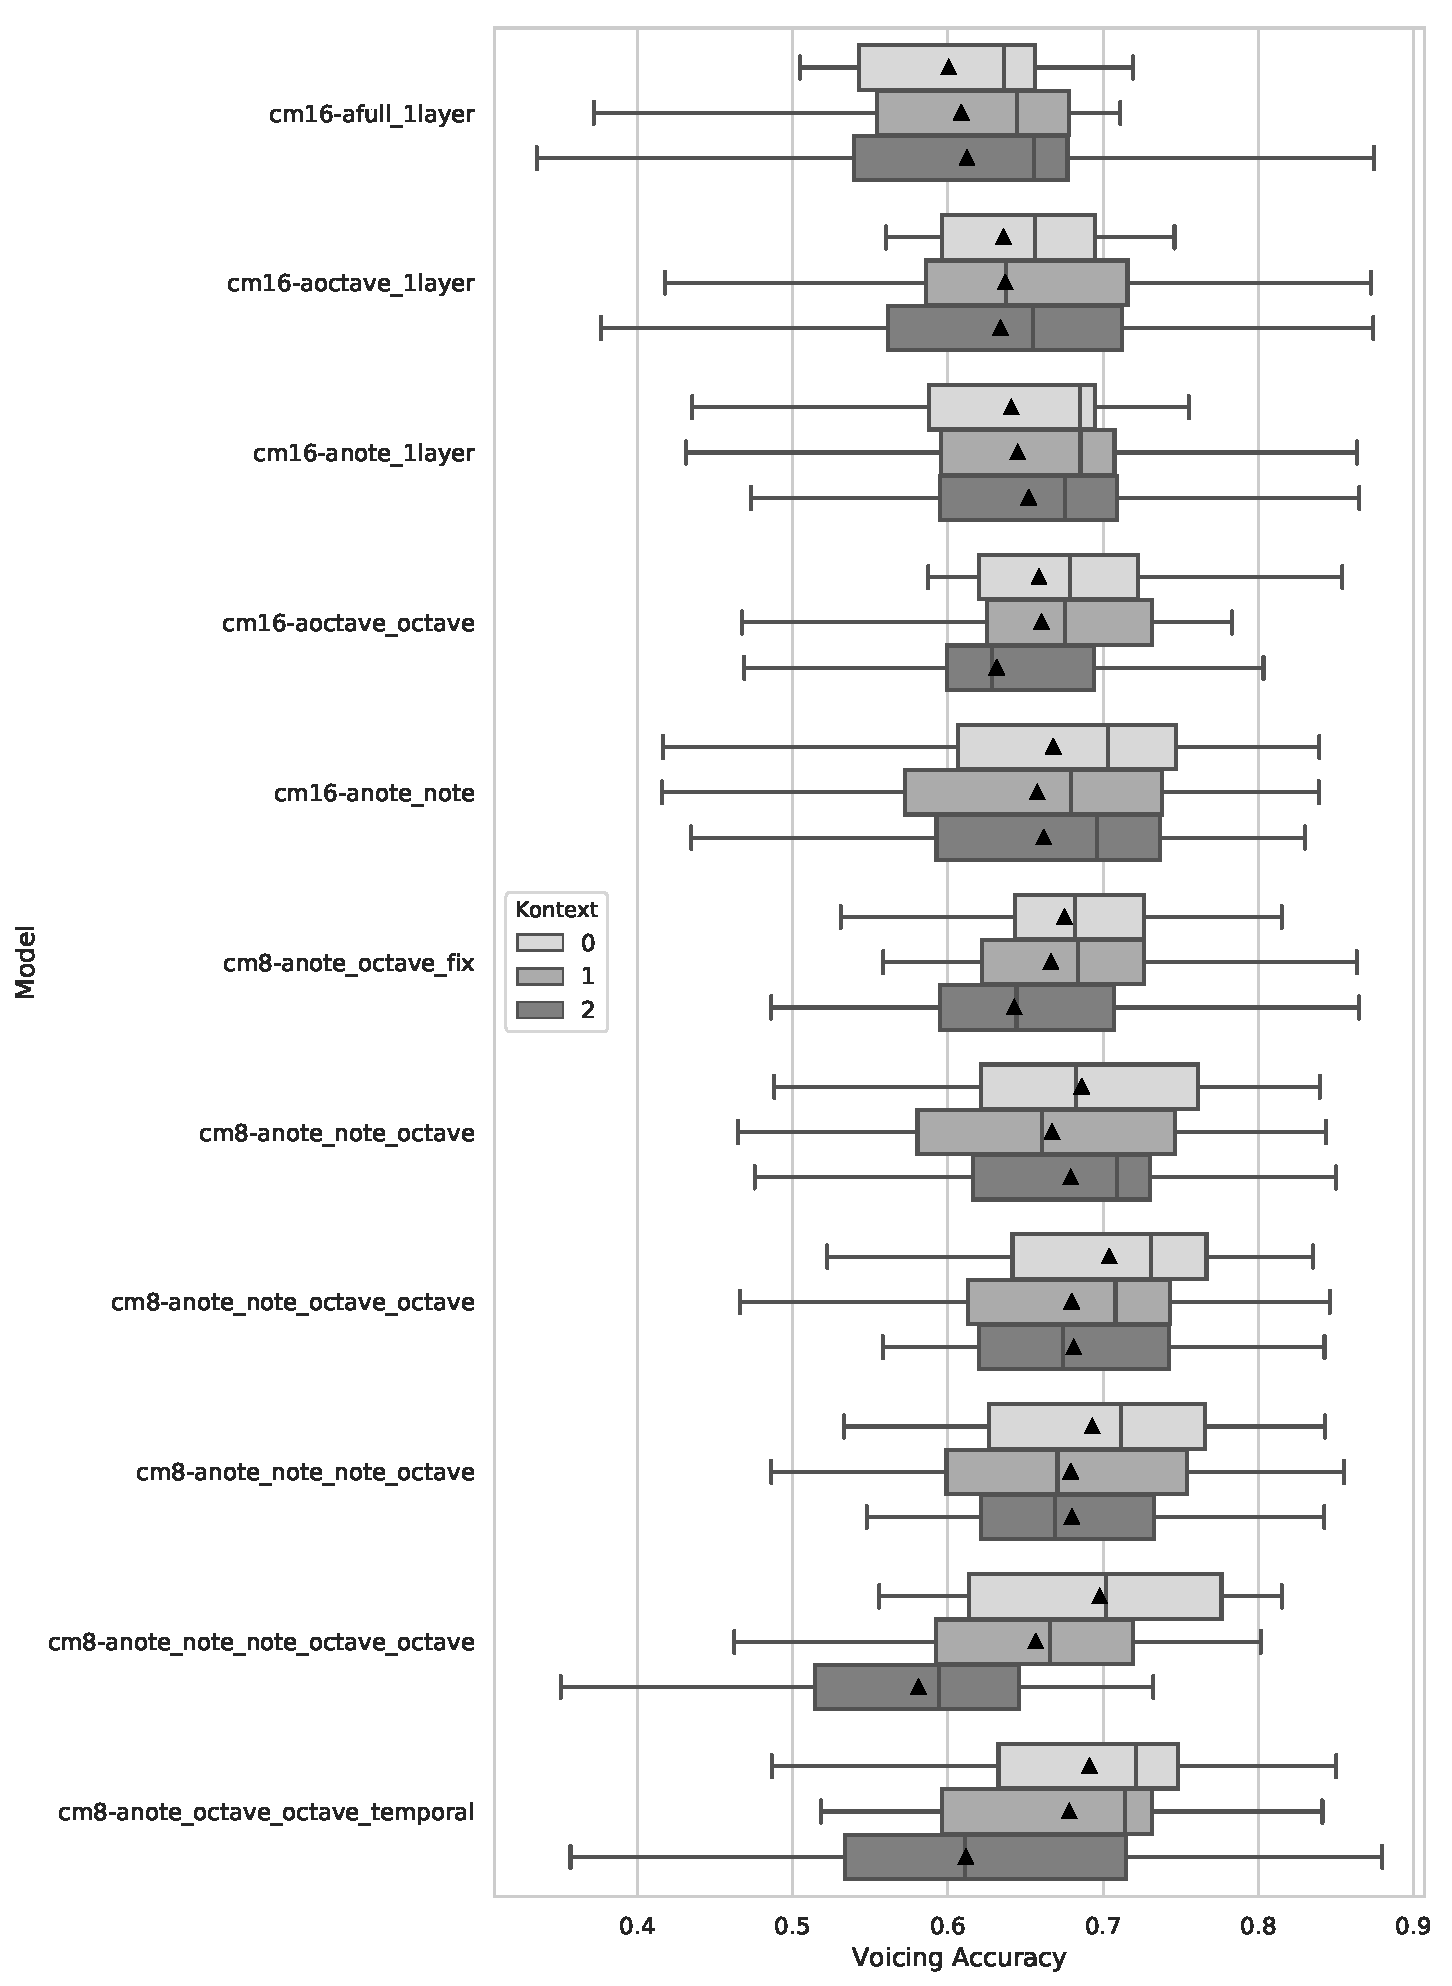
\includegraphics[scale=0.6]{../img/figures/voicing_context_grey}
% \caption{Detekce melodie, vliv kontextu.}\label{obr:voicing_context}
% \end{figure}
